%%
% Copyright (c):
% 	2014-2017 Saúl Piña <sauljabin@gmail.com> (https://github.com/sauljabin/plantilla-latex-trabajo-de-grado-ucla).
% 	2013 Miguel León <melf.ever.after@gmail.com> (https://code.google.com/p/uclamsc).
% 	2009 Juan Rada Vilela <jcrada@gmail.com> y Rubén Parma <parmaia@gmail.com> (https://github.com/jcrada/latex-uclamsc).
%
% This program is free software: you can redistribute it and/or modify
% it under the terms of the GNU General Public License as published by
% the Free Software Foundation, either version 3 of the License, or
% (at your option) any later version.
%
% This program is distributed in the hope that it will be useful,
% but WITHOUT ANY WARRANTY; without even the implied warranty of
% MERCHANTABILITY or FITNESS FOR A PARTICULAR PURPOSE.  See the
% GNU General Public License for more details.
%
% You should have received a copy of the GNU General Public License
% along with this program.  If not, see <http://www.gnu.org/licenses/>.
%%

\documentclass{uclamsc}

\includeonly{
  capitulos/dedicatoria,
  capitulos/agradecimientos,
  capitulos/introduccion,
  capitulos/el-problema,
  capitulos/marco-teorico,
  capitulos/marco-metodologico,
  capitulos/propuesta,
  capitulos/resultados,
  capitulos/conclusiones,
  capitulos/anexos
}

% Bibliografia
\bibliografia{bibliografia}

%% Comandos de identificación

% Sobre el autor
\autor{Ing. Saúl Jabín Piña Alvarado}
\citarcomo{Piña}
% \esautora

% Sobre el trabajo
\titulo{Implementación de un Modelo Afectivo para la Arquitectura Multiagente para Sistemas Auto-Organizados y Emergentes (MASOES)}
\title{Implementation of an Affective Model for the Multiagent Architecture for Self-Organizing And Emergent Systems (MASOES)}
\palabrasclave{Sistemas Multiagente, Computación Emocional, Modelo Afectivo, Interacción Emocional, MASOES}
\keywords{Multiagent System, Affective Computing, Emotional Model, Emotional Interaction, MASOES}
\grado{Magister Scientiarum en Ciencias de la Computación}
\mencion{Mención Inteligencia Artificial}

% Sobre la universidad
\decanato{Ciencias y Tecnología}
\postgrado{Maestría en Ciencias de la Computación}

% Sobre el tutor
\tutor{Dra. Niriaska Perozo Guédez}
\estutora

% Sobre la presentación
\ciudad{Barquisimeto}
\diapresentacion{25}
\mespresentacion{Octubre}
\monthpresentacion{October}
\anopresentacion{2017}
\primerjurado{Prof. José Gregorio Sánches}
\segundojurado{Prof. Sandra Lima}

%% Fin Comandos de identificación

%% Configuraciones especiales

\setnombreilustracion{Figura}{Figuras}
\setnombrecuadro{Tabla}{Tablas}
\numerarsecciones
\tutorenpresentacion

%% Fin Configuraciones especiales

\begin{document}

	%%
% Copyright (c) {año} {nombre} <{email}>.
%
% This program is free software: you can redistribute it and/or modify
% it under the terms of the GNU General Public License as published by
% the Free Software Foundation, either version 3 of the License, or
% (at your option) any later version.
%
% This program is distributed in the hope that it will be useful,
% but WITHOUT ANY WARRANTY; without even the implied warranty of
% MERCHANTABILITY or FITNESS FOR A PARTICULAR PURPOSE.  See the
% GNU General Public License for more details.
%
% You should have received a copy of the GNU General Public License
% along with this program.  If not, see <http://www.gnu.org/licenses/>.
%%

	\resumen{%%
% Copyright (c) {año} {nombre} <{email}>.
%
% This program is free software: you can redistribute it and/or modify
% it under the terms of the GNU General Public License as published by
% the Free Software Foundation, either version 3 of the License, or
% (at your option) any later version.
%
% This program is distributed in the hope that it will be useful,
% but WITHOUT ANY WARRANTY; without even the implied warranty of
% MERCHANTABILITY or FITNESS FOR A PARTICULAR PURPOSE.  See the
% GNU General Public License for more details.
%
% You should have received a copy of the GNU General Public License
% along with this program.  If not, see <http://www.gnu.org/licenses/>.
%%
}
	\abstract{%%
% Copyright (c) 2017 Saúl Piña <sauljabin@gmail.com>.
%
% This program is free software: you can redistribute it and/or modify
% it under the terms of the GNU General Public License as published by
% the Free Software Foundation, either version 3 of the License, or
% (at your option) any later version.
%
% This program is distributed in the hope that it will be useful,
% but WITHOUT ANY WARRANTY; without even the implied warranty of
% MERCHANTABILITY or FITNESS FOR A PARTICULAR PURPOSE.  See the
% GNU General Public License for more details.
%
% You should have received a copy of the GNU General Public License
% along with this program.  If not, see <http://www.gnu.org/licenses/>.
%%

Affective computation is a recent area of the artificial intelligence
that aims to improve the interactive processes between emotional agents and the human,
both for software and hardware applications.
Currently the scientific community makes efforts to apply existing theories in
multiagent systems by potential applications in this area.
Different authors study emotional models in order to improve interaction between intelligent agents,
an example is the affective model of MASOES,
although this affective model has been formally verified at the design level,
it has not been verified at the implementation level.
In light of the above, this paper proposes an implementation of the MASOES affective model on a multiagent system,
in order to provide an environment for the interaction between the emotional processes and the different functions of an agent.
In addition, the calculation of the Social Emotion is proposed,
allowing to describe the collective emotional state of a group of emotional agents.
To achieve this, a multiagent system was designed and developed based on the JADE framework,
which uses the FIPA standard to develop universal agents.
Finally, the implemented was applied on a case of study using simulations
to generate individual and collective emotions,
and the results were compared at the implementation level with those obtained by \cite{perozo2011} at the design level.
}

  \begin{preliminares}
  	\hacercaratula
  	\hacerpresentacion
  	\haceraprobacion
  	%%
% Copyright (c) {año} {nombre} <{email}>.
%
% This program is free software: you can redistribute it and/or modify
% it under the terms of the GNU General Public License as published by
% the Free Software Foundation, either version 3 of the License, or
% (at your option) any later version.
%
% This program is distributed in the hope that it will be useful,
% but WITHOUT ANY WARRANTY; without even the implied warranty of
% MERCHANTABILITY or FITNESS FOR A PARTICULAR PURPOSE.  See the
% GNU General Public License for more details.
%
% You should have received a copy of the GNU General Public License
% along with this program.  If not, see <http://www.gnu.org/licenses/>.
%%

\preliminar{Dedicatoria}

  	%%
% Copyright (c) 2017 Saúl Piña <sauljabin@gmail.com>.
%
% This program is free software: you can redistribute it and/or modify
% it under the terms of the GNU General Public License as published by
% the Free Software Foundation, either version 3 of the License, or
% (at your option) any later version.
%
% This program is distributed in the hope that it will be useful,
% but WITHOUT ANY WARRANTY; without even the implied warranty of
% MERCHANTABILITY or FITNESS FOR A PARTICULAR PURPOSE.  See the
% GNU General Public License for more details.
%
% You should have received a copy of the GNU General Public License
% along with this program.  If not, see <http://www.gnu.org/licenses/>.
%%

\preliminar{Agradecimientos}

A mi madre y padre, por todo su apoyo, esfuerzo y amor, para que logre todas mis metas.

A mi esposa, por toda la ayuda que me brinda en todos mis proyectos y por siempre decirme \comillas{Nunca te rindas}.

A mi hermano, mi mejor amigo, que siempre ha estado ahí para apoyarme en lo que necesite.

A mi tutora Niriaska Perozo, por su asesoría durante el desarrollo de este trabajo, consejos y amistad, que me han permitido lograr este objetivo; he aprendido mucho de ella.

A mis compañeros de maestría, buenos amigos que siempre me han apoyado durante el desarrollo de este trabajo.

A todos los amigos y amigas que me han alentado para concluir esta meta y a todas las personas que colaboraron para que así sea.

  	\hacerindices
  	\hacerresumen
  	\hacerabstract
  \end{preliminares}

  \begin{contenido}
  	%%
% Copyright (c) 2017 Saúl Piña <sauljabin@gmail.com>.
%
% This program is free software: you can redistribute it and/or modify
% it under the terms of the GNU General Public License as published by
% the Free Software Foundation, either version 3 of the License, or
% (at your option) any later version.
%
% This program is distributed in the hope that it will be useful,
% but WITHOUT ANY WARRANTY; without even the implied warranty of
% MERCHANTABILITY or FITNESS FOR A PARTICULAR PURPOSE.  See the
% GNU General Public License for more details.
%
% You should have received a copy of the GNU General Public License
% along with this program.  If not, see <http://www.gnu.org/licenses/>.
%%

\introduccion

Se sabe que las emociones juegan un papel importante en el desarrollo de los
seres humanos para fines sociales o de supervivencia \citep{cuevas2015, rodriguez2015}.
Un objetivo importante planteado por la comunidad científica es
construir sistemas artificiales que exhiben comportamiento emocional, para
mejorar la interacción hombre-máquina. Los procesos emocionales se han
convertido en un requisito esencial en arquitecturas de agentes cognitivos, se
espera que el procesamiento afectivo mejore la calidad y la credibilidad de las
respuestas emocionales generadas por los agentes \citep{rodriguez2015}. Con
la aparición de la computación ubícua \citep{weiser1993} y el internet de las
cosas \citep{ashton2009} la cantidad de dispositivos heterogéneos conectados ha
aumentado considerablemente, y por ende las interacciones entre sí y con los
humanos, haciendo que sea imperativo el desarrollo y aplicación de nuevas
técnicas que permitan una mejor respuesta de estos dispositivos, además,
tengan la capacidad de auto-organizarse, lo que traerá como consecuencia la
simplificación del diseño y la emergencia de estructuras complejas en sistemas
multiagente \citep{perozo2011}.

La computación afectiva es una de las áreas de la inteligencia artificial con
mayor interés debido a las posibles aplicaciones, puede ser usada en
simulaciones de sociedades emocionales como las del ser humano, en el
tratamiento de trastornos como el autismo, el síndrome de Asperger, la
epilepsia y depresión, así como en el reconocimiento de riesgo de estrés y su
mitigación. A su vez, se generan controversiales inferencias
sobre esta rama de la ciencia, se prevé que el impacto en el futuro de la
computación afectiva será un enorme reto para la humanidad, se plantea que es
posible que los computadores emocionales llegarán a integrarse en la sociedad
hasta el punto de necesitar derechos, al igual que los tenemos las personas,
además, la computación emocional podría reemplazar el afecto humano \citep{cuevas2015}.

En la actualidad no se conoce completamente los procesos cerebrales y mentales
asociados a las emociones, sin embargo, se realizan esfuerzos para aplicar las
teorías existentes en sistemas computacionales, diferentes autores estudian
modelos emocionales en sistemas multiagente, esto, con el objetivo de mejorar la
interacción de los agentes y ayudar a la auto-organización y emergencia en
dichos sistemas, además, incorporar emociones a agentes inteligentes
es de utilidad, debido a que las
emociones pueden hacer a los agentes más atractivos y creíbles para que puedan
desempeñar un mejor papel en diversos sistemas interactivos que involucren
simulación \citep{jiang2007}.
Un ejemplo es el modelo afectivo de MASOES \eningles{Multiagent
Architecture for Self-Organizing and Emergent Systems}, propuesto por
\cite{perozo2011}, es un modelo afectivo dimensional el cual considera un conjunto de emociones positivas y
negativas que permiten generar un cambio dinámico de comportamiento en los
agentes a nivel individual (Reactivo, Cognitivo) y colectivo (Imitativo), en
otras palabras, los agentes exhiben un comportamiento asociado a su estado
emocional actual, asimismo, los estímulos internos (Individual) o externos
(Colectivo) afectan el estado emocional de los agentes.
Está compuesto por las dimensiones \textit{activación} y \textit{satisfacción},
la primera representa el grado de activación fisiológica y psicológica del agente,
y la segunda el agrado o desagrado exhibido. Este modelo afectivo
para MASOES ha sido verificado \citep{perozo2011} pero no ha sido implementado,
por tal razón, se propone en este trabajo su implementación en un sistema
multiagente para evaluarlo en la generación de emociones a nivel individual y
colectivo a través de un caso de estudio que se seleccione, a fin de comparar
con los resultados ya obtenidos a nivel de la verificación del diseño.

La presente investigación se encuentra estructurada de la siguiente manera:

Capítulo I: se realiza una descripción del problema a abordar
y se plantean los objetivos de la investigación, además, se incluyen la
justificación y el alcance de la investigación.

Capítulo II: comprende la revisión del estado del arte
sobre sistemas multiagente y modelos afectivos dimensionales, también se presentan las bases
teóricas que sustentan esta investigación.

Capítulo III: el marco metodológico presenta la naturaleza y las fases para llevar a cabo la
investigación.

Capítulo IV: se describe de manera detallada la propuesta planteada a nivel
de diseño e implementación.

Capítulo V: expone los casos de estudio realizados y compara los resultados con los obtenidos a nivel de diseño
por parte de \cite{perozo2011}.

Finalmente, Capítulo 6: se detallan las conclusiones y hallazgos en la presente investigación, así
como posibles trabajos futuros.

  	%%
% Copyright (c) {año} {nombre} <{email}>.
%
% This program is free software: you can redistribute it and/or modify
% it under the terms of the GNU General Public License as published by
% the Free Software Foundation, either version 3 of the License, or
% (at your option) any later version.
%
% This program is distributed in the hope that it will be useful,
% but WITHOUT ANY WARRANTY; without even the implied warranty of
% MERCHANTABILITY or FITNESS FOR A PARTICULAR PURPOSE.  See the
% GNU General Public License for more details.
%
% You should have received a copy of the GNU General Public License
% along with this program.  If not, see <http://www.gnu.org/licenses/>.
%%

\capitulo{El Problema}

\seccion{Planteamiento del Problema}

\seccion{Objetivos}
	\subseccion{Objetivos Generales}
	\subseccion{Objetivos Específicos}

\seccion{Justificación e Importancia}

\seccion{Alcances y Limitaciones}
	\subseccion{Alcances}
	\subseccion{Limitaciones}

  	%%
% Copyright (c) 2017 Saúl Piña <sauljabin@gmail.com>.
%
% This program is free software: you can redistribute it and/or modify
% it under the terms of the GNU General Public License as published by
% the Free Software Foundation, either version 3 of the License, or
% (at your option) any later version.
%
% This program is distributed in the hope that it will be useful,
% but WITHOUT ANY WARRANTY; without even the implied warranty of
% MERCHANTABILITY or FITNESS FOR A PARTICULAR PURPOSE.  See the
% GNU General Public License for more details.
%
% You should have received a copy of the GNU General Public License
% along with this program.  If not, see <http://www.gnu.org/licenses/>.
%%

\capitulo{Marco Teórico}

\seccion{Antecedentes de la Investigación}

La investigación de \cite{rodriguez2015}, es importante para el presente
trabajo ya que plantea cuatro problemas clave que tienen lugar en el desarrollo
de sistemas multiagente con computación emocional, los cuales son: \textit{la
integración de la cognición y las emociones en arquitecturas de agentes, la
unificación de los diversos aspectos de las emociones, arquitecturas escalables
para los modelos computacionales de emociones y la explotación de la evidencia
biológica}. La integración de la cognición y las emociones en arquitecturas de
agentes, se refiere a que las arquitecturas deben proporcionar entornos
adecuados para la interacción de las funciones cognitivas y afectivas que
intervienen en los procesos emocionales, en otras palabras, la construcción
interna de los agentes debe asegurar un correcto acoplamiento entre los
diferentes componentes y el componente afectivo. La unificación de los diversos
aspectos de las emociones, teniendo en cuenta que no existe una teoría universal
que explique todo el proceso de las emociones humanas y que todos los sistemas
afectivos artificiales son desarrollados basándose en los supuestos de dichas
teorías, las arquitecturas afectivas deben proporcionar marcos adecuados para la
aplicación coherente de diferentes aspectos de las emociones humanas. El
problema de las arquitecturas escalables, viene dado a que las investigaciones y
el conocimiento de las emociones humanas se encuentran en constante cambio, las
arquitecturas afectivas deben ser diseñadas de una manera flexible para que
puedan incorporar nuevos componentes y comportamientos, y de esa manera incluir
los nuevos hallazgos. Por último, el problema de la explotación de evidencia
biológica, se refiere a que las arquitecturas deben ser diseñadas de manera que
puedan aprovechar al máximo el conocimiento generado en otras áreas científicas,
además, deben incluir una serie de componentes que imitan el funcionamiento de
las estructuras del cerebro implicadas en el procesamiento de las emociones
humanas. El presente trabajo de investigación
se enfoca en dar solución al primer problema (\textit{la
integración de la cognición y las emociones en arquitecturas de agentes}),
ya que la arquitectura individual de MASOES
describe los componentes y relaciones internas de los agentes emocionales,
para producir y priorizar un comportamiento imitativo, cognitivo o reactivo
guiado por el componente afectivo.

Sobre la arquitectura MASOES se pueden mencionar las siguientes investigaciones:

La arquitectura multiagente para sistemas emergentes y auto-organizados llamada
MASOES \eningles{Multiagent Architecture for Self-Organizing and Emergent Systems},
fue introducida por \citeauthor{perozo2011} en \citeyear{perozo2011}, como una arquitectura
multiagente para el diseño, modelado y estudio de sistemas emergentes y
auto-organizados, más recientemente ha sido utilizada entre otras cosas para
modelar el fenómeno de la auto-organización y emergencia en Wikipedia \citep{perozo2013},
desarrollo de software libre \citep{perozo2013} y sistemas
multirobot \citep{gil2015}. Esta arquitectura describe los elementos,
relaciones y mecanismos, a nivel individual y colectivo, que determinan los
fenómenos de emergencia y auto-organización en un sistema, sin modelar
matemáticamente el mismo. Uno de los aspectos más interesantes de la
arquitectura MASOES, es el hecho de considerar un conjunto de emociones
positivas y negativas generadas desde un nivel individual y colectivo, para de
esta manera promover un cambio de comportamiento dinámico en los agentes en lo
individual (Reactivo, Cognitivo) como colectivo (Imitativo). Dicha
investigación, es muy importante debido a que plantea el modelo afectivo para
MASOES, el cual será utilizado en la presente investigación como base
fundamental para la construcción de una arquitectura multiagente con agentes
emocionales.

En este sentido el trabajo realizado por \cite{gil2015}, también es clave en
el área y para este trabajo, porque demuestra la aplicabilidad de los sistemas
multiagente con modelos emocionales en un problema específico, en este caso
sistemas multirobot (a nivel de hardware). La investigación usa como base el
modelo MASOES propuesto por \cite{perozo2011}. En su investigación proponen una
arquitectura con tres niveles, el primer nivel individual proporciona las
capacidades perceptivas a cada agente y los aspectos relacionados a la conducta
y emociones del robot. El segundo nivel es colectivo, soporta los procesos de
interacción de los robots con otros individuos dentro del sistema y con el medio
ambiente. El último nivel, de los procesos de aprendizaje y gestión del
conocimiento, gestiona el conocimiento tanto individual como colectivo, así como
los procesos de aprendizaje que se producen en el sistema.

Por otra parte, también es necesario mencionar otras arquitecturas y modelos
afectivos recientes enfocados en el aspecto cognición-emoción que pueden
contribuir a la implementación y evaluación de este trabajo de investigación:

La arquitectura afectiva FATIMA \eningles{Fearnot AffecTIve Mind Architecture},
propuesta por \cite{dias2014}, es una arquitectura para la
generación de emociones en agentes de software, de manera que dichas emociones
afecten el comportamiento del mismo. En este trabajo se utiliza como primera
aproximación para la generación y evaluación de emociones el modelo afectivo OCC
\eningles{Ortony, Clore and Collins} \citep{ortony1990},
en este modelo se presentan las emociones de manera categorizada y no a través
de dimensiones como otros estudios. El proceso de evaluación de las emociones se
realiza en dos pasos, en primer lugar se determina la importancia de un evento
para el agente y se definen las variables de valoración del evento,
posteriormente, se toman las variables y se genera como resultado el estado
afectivo, el cual permite cambiar el comportamiento del agente. Cada emoción
poseerá un valor, tipo y una intensidad, el estado de ánimo del agente se puede
definir como el estado afectivo general, que está influenciado por las emociones
experimentadas por el agente, las emociones positivas aumentan el estado de
ánimo, mientras que las emociones negativas lo disminuyen. En esta investigación
no se establece una relación entre las emociones y el comportamiento, como lo
realiza el modelo afectivo para MASOES, en cambio, se muestra la relación entre
las variables de valoración  y las emociones, dicha relación es extraída de la
categorización OCC: \textit{la variable deseabilidad se relaciona con alegría y
angustia, la plausibilidad con rechazo, admiración, orgullo y vergüenza, la
capacidad de atracción con amor y odio, entre otros}. En esta arquitectura se
toma en cuenta el estado emocional que puede ser producido por agentes externos
y por el ambiente, y además se habla de un componente cultural, que está
directamente relacionado con la variable plausibilidad, puede darse el caso que
entre más positiva sean las emociones colectivas del agente, es más posible que
priorice acciones positivas para otros agentes y no  para él. Una importante
diferencia con el modelo afectivo para MASOES, es que este promueve un
compromiso entre el comportamiento individual y colectivo en la sociedad de
agentes,  además, permite explicar aspectos de la interacción social, tales como
el grado de satisfacción, cooperación y competencia, entre otros, mientras que
FATIMA, posee un enfoque cognitivo emocional.

\cite{dastani2014programming}, proponen extender el lenguaje de programación de agentes inteligentes llamado \comillas{2APL},
con el objetivo de integrar emociones en este.
2APL es un lenguaje de programación lógico que fue desarrollado para apoyar la programación de sistemas multiagente.
Entre otras cosas, este lenguaje le permite a los agentes recibir eventos y representar información
propia, de otros agentes o del entorno.
Posee un conjunto de tres tipos de reglas de razonamiento:
el primer tipo de reglas está diseñado para generar planes para alcanzar metas,
llamadas reglas de planificación de objetivos o reglas PG \eningles{Planning Goal};
el segundo permite procesar eventos externos, mensajes y acciones abstractas,
llevan el nombre de reglas de llamada de procedimiento o reglas de PC \eningles{Procedure Call};
el último tipo permite rehacer los planes fallidos,
llamadas reglas de reparación del plan o RP \eningles{Plan Repair}.
Con respecto a la integración de emociones, se utilizó
el modelo dimensional de emociones PAD \eningles{Pleasure, Arousal and Dominance},
específicamente la implementación llamada ALMA \eningles{A Layered Model of Affect} \citep{gebhard2005alma}, para definir
el conjunto de emociones que pueden exhibir los agentes, además,
crearon una base de emociones a través de un nuevo tipo de regla para el lenguaje 2APL,
llamadas reglas de emoción o ER \eningles{Emotion Rule}, en las que se definen eventos, acciones u objetos
y la intensidad con que afectarán el estado emocional del agente.
La intensidad puede ser variada por evento,
la idea es que cada evento pueda tener su propio valor
y afecte de diferente manera a la emoción.
Esta investigación sirve de inspiración para el presente trabajo,
ya que guarda similitudes con la arquitectura individual propuesta
en MASOES, en la que se tiene una Base de Conocimiento Conductual,
un Modelo Afectivo Dimensional y se procesan eventos, acciones u objetos para generar emociones.
Además, sirve como base para justificar el uso del
lenguaje de programación lógico \textit{Prolog} en la implementación
propuesta y así definir
el conocimiento asociado a los agentes, emociones,
comportamientos, eventos, acciones u objetos que afectarán las emociones.

\cite{rincon2015}, plantea un modelo afectivo en tres dimensiones llamado SEM
\eningles{Social Emotional Model} basado en el modelo
psicológico de estados emocionales PAD \eningles{Pleasure, Arousal and Dominance},
el cual está definido por las dimensiones placer,
excitación y dominio respectivamente. En el modelo, el placer representa la
medida de cuan agradable se puede sentir una emoción, la excitación mide la
intensidad de lo que se está sintiendo, y el dominio se refiere al control que
ejerce sobre el comportamiento un estado emocional. Al igual que el modelo
propuesto por \cite{perozo2012}, este modelo afectivo SEM utiliza valores
normalizados en un intervalo de [-1,1] para cada dimensión, con la diferencia
que el modelo afectivo de MASOES está fundamentado en un espacio en dos
dimensiones. Ambos modelos consideran emociones individuales y grupales, difiere
en que MASOES tiene como objetivo modelar la auto-organización y emergencia en
un sistema, utilizando el modelo afectivo para que cada agente pueda cambiar su
comportamiento dinámicamente, guiado por su estado emocional para satisfacer
los objetivos del sistema a través de la auto-organización de sus
actividades, mientras que SEM se centra en estudiar los estados emocionales
individuales y grupales a través del tiempo. SEM como modelo afectivo es medible
a nivel colectivo a través de una ecuación que se propone en el trabajo, en
cambio, el modelo afectivo para MASOES se centra en promover un cambio de
comportamiento dinámico e incentivar la interacción social para medir el grado
de auto-organización y emergencia alcanzado por el sistema. Esta capacidad para
caracterizar las interacciones sociales, diferencia a MASOES de otros modelos
emocionales que se centran normalmente en el estudio de la relación
cognición-emoción. De esta manera, ambos modelos son perfectamente aplicables en
simulaciones de sistemas sociales emocionales y además sobre sistemas
multiagente compuestos netamente por agentes de software.
El trabajo de \citeauthor{rincon2015}
resulta útil ya que sirve como base para la propuesta de Emoción Social descrita en esta investigación.

Otro enfoque interesante es presentado por \cite{yu2015}, que propone una
arquitectura denominada EMARL \eningles{Emotional Multiagent Reinforcement Learning},
con el objetivo de dotar a agentes inteligentes de
capacidades cognitivas y emocionales internas que pueden conducir a aprender
comportamientos cooperativos. Un aspecto relevante de este estudio es el
utilizar las emociones como un mecanismo de aprendizaje de comportamientos que
permita a los agentes la maximización de recompensas y la minimización de los
castigos. Ambas arquitecturas, MASOES y EMARL, consideran el comportamiento
colectivo como el resultado de interacciones locales de los agentes de software,
con la diferencia que MASOES utiliza las emociones para ayudar a la generación
de conocimiento colectivo de manera cooperativa, en cambio, EMARL posee un
enfoque llamado dilemas sociales, donde los agentes como entidad individual
deben decidir entre tomar acciones para obtener un beneficio propio a corto
plazo de manera egoísta o cooperar con otros agentes para obtener algún
beneficio a largo plazo. Se puede resaltar de esta arquitectura el modelo
emocional a doble capa, en la capa interna, dos funciones de derivación
emocional compiten entre sí con el fin de dominar el proceso emocional del
agente, mientras que en la capa externa una estrategia explícita de
comportamientos puede ser aprendida en base a la función de derivación emocional
ganadora. En comparación, MASOES divide su modelo afectivo en cuatro fases:
clasificación de emociones, asociación de emociones a tipos de comportamiento,
determinación de la emoción actual y determinación del tipo de comportamiento.
Un importante punto de comparación es el tipo de comportamiento que promueven
estas arquitecturas, en EMARL, se habla de comportamientos altruistas, donde los
agentes cooperan con otros, y el comportamiento egoísta donde el agente busca
satisfacer sus metas individuales, ambos comportamientos son llevados a cabo
según las metas del agente y según el beneficio que pueda obtener (dilemas
sociales), en MASOES, si se trata de una emoción positiva el agente asumirá un
comportamiento imitativo, para llevar a cabo una acción colectiva, en caso de
una emoción negativa, el agente asumirá un comportamiento reactivo o cognitivo,
para llevar a cabo una acción individual.

\seccion{Bases Teóricas}

\subseccion{Sistemas Multiagente}

La Inteligencia Artificial Distribuida (IAD) es una subárea de la Inteligencia
Artificial que ha ganado una considerable importancia debido a su capacidad de
resolver problemas complejos \citep{balaji2010}, está dividida en dos
disciplinas \citep{bond1989}, la Resolución de Problemas Distribuidos (RPD)
y los Sistemas Multiagente (SMA). La RPD considera que un problema puede ser
dividido en varios módulos, o nodos, que cooperan y comparten el conocimiento de
que disponen, quedando toda la interacción entre los nodos prefijada en tiempo
de diseño como parte integrante del sistema. Por otra parte, un SMA se puede
definir como una red de solucionadores de problemas (agentes) con un nivel muy
bajo de acoplamiento, que trabajan conjuntamente, lo que posibilita que se
enfrenten a problemas más complejos que los abordables de forma individual
\citep{perozo2011}. Los agentes autónomos y los sistemas multiagente representan una
nueva forma de analizar, diseñar e implementar sistemas de software complejos.
El enfoque basado en agentes ofrece herramientas y técnicas que tienen el
potencial de mejorar considerablemente la forma en que se conceptualizan e
implementan muchos tipos de software \citep{jennings1998}.

Según \cite{balaji2010}, el concepto más aceptado de Agente es el dado
por \cite{russell2004}, ellos definen un agente como cualquier cosa capaz
de percibir su medioambiente con la ayuda de sensores y actuar sobre él
utilizando actuadores. Por otra parte, para \cite{weiss1999}, un agente es un
sistema computacional que está situado en un ambiente, y que es capaz de tomar
acciones autónomas en ese ambiente con el fin de cumplir sus objetivos de
diseño. Para hablar de agentes inteligentes es necesario que estos estén dotados
de mecanismos de razonamiento que les permiten abordar situaciones de manera
inteligente y evolucionar por medio de la experiencia \citep{perozo2011}.

Entre las propiedades más resaltantes de los agentes inteligentes se encuentran \citep{perozo2011}:

\begin{enumerate}
\item \textbf{Autonomía:} Los agentes son autónomos en la medida en que actúan sin la
intervención humana ni de otros sistemas externos. Sin embargo, un agente
inteligente puede crear redes colaborativas con otros agentes según sus
necesidades. Esta propiedad está muy relacionada a la proactividad.
\item \textbf{Comunicación:} Los agentes tienen la capacidad de comunicarse con otros agentes
utilizando un lenguaje basado en ontologías o realizar intervenciones asíncronas
a través de comunicación indirecta.
\item \textbf{Movilidad:} Es la habilidad del agente de
moverse en el ambiente. Esta capacidad posibilita una computación menos
centralizada y más distribuida. Un agente puede alojarse en cualquier nodo de la
red y realizar sus tareas utilizando los recursos locales, para después volver a
su nodo origen llevando la información procesada.
\item \textbf{Racionalidad:} Se refiere a
que los agentes prefieren ejecutar la acción más prometedora o eficiente para
conseguir sus metas.
\item \textbf{Inteligencia:} El agente está provisto de diferentes
técnicas de inteligencia artificial, que le permiten analizar situaciones
dinámicas
\item \textbf{Razonamiento:} Es la capacidad que tiene un agente para seleccionar
comportamientos acordes a la situación actual, con la finalidad de perseguir,
detener o en su defecto abandonar un objetivo, esta propiedad está muy
relacionada con la inteligencia.
\item \textbf{Sociabilidad:} Los agentes interactúan con
otros agentes mediante algún tipo de comunicación y convenios colectivos. Esta
propiedad está muy relacionada a la cooperación, colaboración y competencia.
\end{enumerate}

Entre las características más representativas de los SMA se pueden mencionar
\citep{schweitzer2007}:

\begin{enumerate}
\item \textbf{Modularidad:} En los SMA, una distinción lógica es hecha entre los módulos y
sus interacciones. Módulos particulares (entidades, subsistemas) de un sistema
son representados por los agentes respectivos. Dependiendo de la granularidad
del modelo, cada uno de esos módulos puede estar compuesto de módulos más
pequeños. Es diferente desde un punto de vista monolítico, que trata al sistema
como un todo. Un punto de vista modular permite la reconfiguración y
extensibilidad del SMA de una manera más fácil.
\item \textbf{Redundancia:} Un SMA consiste
generalmente de un gran número de agentes, muchos de ellos similares en función
y diseño. Esto significa, por un lado, que las instancias críticas no son
representadas por un solo agente, y por otro lado, que el sistema no se cae si
un agente falla de alguna manera, brindándole robustez al sistema.
\item \textbf{Descentralización:} Un SMA no es regido por un control centralizado. En lugar de
eso, las competencias y capacidades, entre otras cosas, son distribuidas entre
los diversos agentes. Esto les permite crear un control \textit{bottom-up}, de una
manera auto-organizada, como resultado de la interacción entre los diferentes
agentes.
\item \textbf{Comportamiento Emergente:} En un SMA, la interacción entre los
agentes puede producir un comportamiento nuevo (y estable) en el nivel global de
todo el sistema. Esto representa una nueva cualidad que resulta del
comportamiento agregado de los agentes, y por lo tanto, no puede ser reducido a
los agentes individuales. Además, debido a los efectos no lineales, es
frecuentemente difícil predecir las propiedades emergentes del sistema a partir
de las propiedades individuales.
\item \textbf{Funcionalidad:} Aunque cada agente puede
tener sus propias funciones (o \textit{comportamientos}), la funcionalidad del sistema
como un todo, por ejemplo, la resolución de un problema, no es asignado a
agentes específicos sino que resulta de la interacción de los diferentes
agentes.
\item \textbf{Adaptación:} La modularidad, la descentralización y la funcionalidad
emergente son las bases para que el SMA se adapte a situaciones cambiantes. Aquí
el exceso de capacidad provista por los agentes redundantes pueden jugar un rol
importante también. Como en la evolución natural, esta asegura una reserva que
puede ser utilizada en situaciones imprevistas, es decir, para la exploración de
nuevas posibilidades u oportunidades, sin perder la funcionalidad del sistema.
La adaptación (algunas veces llamada aprendizaje colectivo) también necesita que
el sistema pueda olvidar/desaprender sus viejos estados e interacciones, entre
otras cosas, para adaptarse a nuevas situaciones.
\end{enumerate}

Dependiendo de la manera de abordar la construcción del agente, existen algunas
arquitecturas clásicas o comunes \citep{perozo2011}:

\begin{enumerate}
\item \textbf{Arquitecturas Reactivas:} Proponen un enfoque conductista, siguiendo un modelo
estímulo-respuesta, y están formadas generalmente por agentes puramente
reactivos.
\item \textbf{Arquitecturas Deliberativas:} Contiene un modelo del mundo
simbólico y explícitamente representado. La toma de decisiones se realiza por
medio de razonamiento simbólico. Está formada por agentes basados en metas o en
la utilidad.
\item \textbf{Arquitecturas Híbridas:} Surgen a partir de numerosas
alternativas que intentan combinar lo mejor de las arquitecturas deliberativas y
reactivas.
\end{enumerate}

\subseccion{Computación Emocional}

El concepto fue introducido por \cite{picard1995}, y el objetivo de la
línea de investigación es lograr una interacción humano/computadora más
eficiente. La afectividad es una dimensión significativa del comportamiento y la
comunicación humana. Lograr que las computadoras puedan comprender nuestras
emociones y a la vez que puedan \textit{expresar} (o simular) emociones propias, sería
un paso importante para establecer un cambio cualitativo en la interactividad.
La Computación Afectiva \eningles{Affective Computing} o Computación
Emocional es una disciplina de la Inteligencia Artificial que intenta
desarrollar métodos computacionales orientados a reconocer emociones humanas y
generar emociones sintéticas \citep{causa2008}.

Según \cite{causa2008}, la computación afectiva se ocupa en resolver las
siguientes problemáticas:

\begin{enumerate}
\item El reconocimiento de emociones (y de expresiones emotivas)
humanas por parte de una computadora. El objetivo es captar aquellos signos
relacionados con la expresión de emociones y lograr interpretar estados
emocionales en función de dichos signos. Este es un tema muy complejo en el que
es difícil obtener precisión. De hecho, no existe una terminología
universalmente consensuada a la hora de referirse a estos fenómenos.
\item La simulación (o generación) de estados y expresiones emocionales con computadoras.
Se intenta que las computadoras puedan simular procesos emocionales en base a
ciertos modelos. Aquí se puede reflexionar respecto a si una computadora puede
realmente tener emociones, pero esta disciplina solo intenta simular dichos
procesos de forma tal que resulten verosímiles, dejando de lado estas
controversias.
\end{enumerate}

Con respecto a los agentes inteligentes, hay muchas razones para incorporar las
emociones \citep{jiang2007}. Las emociones pueden hacer a los agentes más
atractivos y creíbles para que puedan desempeñar un mejor papel en diversos
sistemas interactivos que involucren simulación. Las emociones pueden jugar un
papel funcional en el comportamiento de los seres humanos y los animales,
particularmente en sistemas sociales complejos, las emociones pueden modificar
el comportamiento físico de los agentes: un agente feliz se mueve más rápido,
mientras que un agente triste es más lento. Por otra parte, los estados
emocionales pueden afectarse según el éxito o el fracaso de metas, o de manera
inversa el estado emocional puede afectar el cumplimiento de los objetivos.
Además, las emociones pueden influir en los procesos de supervivencia del
agente, evitando situaciones riesgosas o que no cumplan con sus objetivos.

Específicamente, podemos mencionar algunos roles potenciales para las emociones
en los agentes artificiales \citep{maria2007}:

\begin{enumerate}
\item \textbf{Selección de Acciones:} Que hacer próximamente en base al estado emocional
actual.
\item \textbf{Adaptación:} Cambios en el comportamiento a corto y largo plazo debido
a los estados emocionales.
\item \textbf{Regulación Social:} Comunicación o intercambio de
información con otros vía expresiones emocionales.
\item \textbf{Integración Sensorial:} Filtrado de datos en función del estado de las
emociones y el entorno.
\item \textbf{Mecanismos de Alarma:} Reacciones, como reflejos rápidos, en situaciones críticas
que interrumpen otros procesos.
\item \textbf{Motivación:} Creando motivos como parte de un
mecanismo de imitación-emoción.
\item \textbf{Manejo de Metas:} Creación de nuevas metas o
repriorización de las existentes.
\item \textbf{Aprendizaje:} Evaluaciones emocionales en el
aprendizaje por refuerzo.
\item \textbf{Centrar la atención:} Selección de datos a procesar
basados en la evaluación emocional.
\item \textbf{Control de Memoria:} Acceso, recuperación
y disminución de elementos en memoria según estados emocionales.
\item \textbf{Procesamiento estratégico:} Selección de diferentes métodos de búsqueda basada en
el estado emocional general.
\item \textbf{Auto-modelo:} Emociones que representan como experimenta una situación un agente.
\end{enumerate}

\subseccion{MASOES}

La arquitectura multiagente para sistemas emergentes y auto-organizados llamada
MASOES \eningles{Multiagent Architecture for Self-Organizing and Emergent Systems},
propuesta por \cite{perozo2011}, es una herramienta para el diseño no
formal de sistemas, que produzcan un estado auto-organizado el cual emerja de
las interacciones locales entre los agentes y de los cambios que se dan en el
entorno. En esta arquitectura, cada agente puede cambiar su comportamiento
dinámicamente, guiado por su estado emocional, para satisfacer los
objetivos del sistema a través de la auto-organización de sus actividades.

\subsubseccion{Niveles de Interacción de MASOES}

La emergencia cognitiva colectiva es obtenida a través de tres diferentes
tipos de interacción \refpilustracion{arquitectura-multiagente-masoes}:

\begin{enumerate}
\item \textbf{Interacción Local:} Es el dinamismo e influencia (interdependencia)
estrictamente entre agentes (directa, a través de alguna forma de comunicación),
o entre agentes y el entorno (indirecta, usando un campo de acción que permite
la delimitación de un área común siguiendo un mismo conjunto de reglas).
\item \textbf{Interacción Grupal:} Es originada por el dinamismo de las interacciones locales
para favorecer la creación de redes sociales o grupos estructurados de acuerdo a
un objetivo colectivo, apoyando la gestión del conocimiento de una manera
comunitaria y colaborativa.
\item \textbf{Interacción General:} Es el resultado de la interacción de la comunidad de
agentes involucrados en el sistema conforme a los objetivos comunes.
\end{enumerate}

\begin{ilustracion}[fuente=\cite{perozo2011}, etiqueta=arquitectura-multiagente-masoes, titulo={Arquitectura de MASOES}]
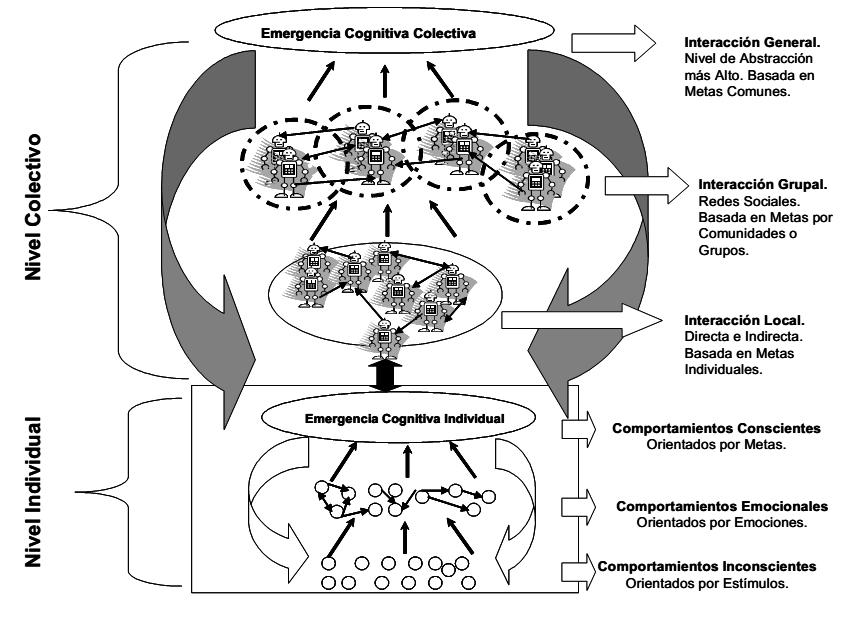
\includegraphics[width=10cm]{ilustraciones/marco-teorico/arquitectura-multiagente-masoes.jpg}
\end{ilustracion}

\subsubseccion{Comportamientos de los Agentes}

\begin{enumerate}
\item Comportamiento Inconsciente o reactivo, según estímulos.
\item Comportamiento Emocional, orientado por las emociones.
\item Comportamiento Consciente, que se activan o inhiben en función de sus objetivos.
\end{enumerate}

Las emociones son usadas como un mecanismo de toma de decisiones para evaluar si
el comportamiento reactivo, cognitivo o imitativo es más conveniente o no para
una situación dada de acuerdo a los intereses individuales y colectivos.

\subsubseccion{Componentes de MASOES a Nivel Colectivo}

Los componentes a nivel colectivo son los siguientes \refpilustracion{componente-masoes}:

\begin{enumerate}
\item \textbf{Conjunto de reglas:} especifican las interacciones
entre los agentes usando solamente información local.
\item \textbf{Entorno:} es un elemento importante para las interacciones indirectas entre los agentes y
para la recolección de la información generada por la sociedad de agentes.
\item \textbf{Campo de Acción:} es delimitada por los agentes, a través de marcas
dejadas en el entorno, generalmente para coordinar sus comportamientos. En
general, existen dos tipos de coordinación entre agentes: coordinación por
comunicación directa y coordinación dentro de campos de acción (comunicación
indirecta).
\item \textbf{Base de Conocimiento Colectivo:} es la memoria social
o colectiva a la que todos los agentes tienen acceso.
\item \textbf{Retroalimentación positiva:} para promover la creación de estructuras y
cambios en el sistema.
\item \textbf{Retroalimentación negativa:} para compensar
la retroalimentación positiva y ayudar a estabilizar el patrón de comportamiento
colectivo.
\end{enumerate}

\begin{ilustracion}[fuente=\cite{perozo2011}, etiqueta=componente-masoes, titulo={Componentes de MASOES a Nivel Colectivo}]
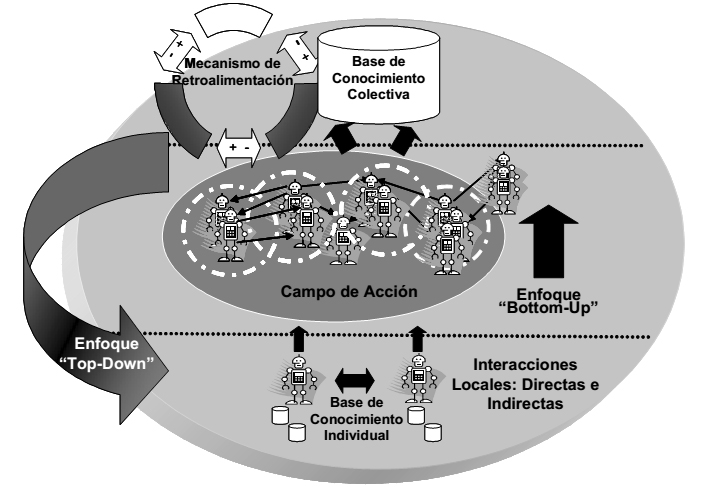
\includegraphics[width=10cm]{ilustraciones/marco-teorico/componente-masoes.jpg}
\end{ilustracion}

\subsubseccion{Componentes de MASOES a Nivel Individual}

La arquitectura a nivel individual tiene 4 componentes: Conductual (procesos
emocionales y de cambio de comportamiento o comportamientos orientados por
emociones), Reactivo (procesos reactivos o comportamientos inconscientes),
Cognitivo (procesos deliberativos o comportamientos conscientes) y Social
(procesos sociales o comportamiento social) \refpilustracion{componentes-masoes-individual}.

\begin{enumerate}
\item \textbf{Componente Conductual:} Favorece la adaptación de cada agente con su
entorno ya que crea un modelo interno del mundo exterior que regula su
comportamiento de una manera consciente y emocional. Cada proceso de toma de
decisiones en el agente estará basado en sus objetivos individuales y
colectivos, su estado emocional, y el conocimiento adquirido de manera
individual y colectiva. Los tipos de comportamiento a considerar son imitar,
reaccionar y razonar, los cuales están enlazados a los componentes social,
reactivo y cognitivo, respectivamente. Entre los elementos que lo conforman está
el Configurador Emocional encargado de manipular las emociones del agente. En
este caso, las emociones son consideradas como señales y evaluaciones que
informan, modifican y reciben retroalimentación de los procesos reactivos,
cognitivos y sociales (de otros agentes), es en este sub-componente donde estará
el modelo afectivo. También está el Manejador de Comportamiento o Conductual,
que se encarga de activar, inhibir y priorizar algunos comportamientos en el
agente basado en el estado emocional actual, las metas del agente, su situación
social (situación de sus vecinos más cercanos) y el entorno en general. Además,
maneja todos los mecanismos responsables del cambio dinámico de comportamiento,
ya que su objetivo principal es determinar y sugerir un único tipo de
comportamiento cada vez para evitar conflictos en tiempo de ejecución. El
conocimiento asociado con la gestión de las emociones, comportamientos y
experiencias emocionales pasadas, es almacenado en la Base de Conocimiento (BC)
Conductual. El rol de las emociones es determinar el comportamiento del agente
según su estado emocional, para ello se asocian las clases de emociones a
considerar con los tipos de comportamiento que puede presentar el agente.
\item \textbf{Componente Reactivo:} Encargado de producir el comportamiento reactivo del
agente. Las reacciones son reglas asociadas a los estados emocionales ya que, se
quiere tener algunas reglas activas y otras no, de acuerdo al estado emocional
del agente y a la actividad que desarrolla en un momento determinado. Para ello
tiene un Selector de Reacciones que selecciona entre las diferentes rutinas de
comportamiento existentes, es decir, las que serán ejecutadas por el componente
reactivo de acuerdo con el estado emocional del agente. Además, posee una BC
Reactivo que es la base de conocimiento reactivo para almacenar el conjunto de
reglas gestionadas por el componente reactivo.
\item \textbf{Componente Cognitivo:} Es el responsable de producir el comportamiento
cognitivo a través de diversos mecanismos cognitivos (aprendizaje y
razonamiento), y procesos de toma de decisión (intencional o deliberativa, entre
otras). Posee un Configurador de Metas Individuales para la configuración de los
objetivos individuales y de las prioridades del agente; un Deliberador como
responsable de los mecanismos cognitivos (aprendizaje, razonamiento) y de la
toma de decisión intencional o deliberativa, entre otras; y una BC Cognitiva.
\item \textbf{Componente Social:} Debe promover conciencia en los agentes sobre el
trabajo y la experiencia de los otros agentes. Específicamente, aprovecha la
experiencia de los otros (aprendizaje social), es decir, evita el aprendizaje de
cosas que ya han aprendido sus vecinos. Este componente conecta el aprendizaje
colectivo colaborativo con el aprendizaje individual. Para ello tiene un
Configurador de Metas Colectivas para la configuración de los objetivos
colectivos y de las prioridades de los agentes. También tiene una BC Social para
almacenar, entre otras cosas, el conocimiento sobre las decisiones tomadas por
sus vecinos, es decir los agentes más cercanos. Finalmente posee un Razonador
Social para seleccionar que acción debe ser imitada y de cual agente, basado en
las metas colectivas y la utilidad obtenida en casos anteriores. La idea
principal es que cada agente pueda aprender del colectivo.
\item \textbf{Otros Elementos Generales:} Tiene un Sistema de Entrada que provee a los
agentes de información sobre el mundo donde viven. Este sistema pasa las
percepciones recibidas de manera paralela al componente reactivo, conductual,
cognitivo y social. Todos los componentes interactúan recíprocamente con esa
entrada, pero es el componente conductual el que debe establecer cual componente
tiene la prioridad más alta para responder. Posee también un conjunto de
Acciones, que son las reglas de condición-acción (si... entonces) usadas en un
proceso deliberativo (ellas reflejan el comportamiento reactivo y/o cognitivo).
Finalmente, tiene un Sistema de Salida para elegir la acción del componente
indicado por el manejador conductual, en el caso que existan varias respuestas.
\end{enumerate}

\begin{ilustracion}[fuente=\cite{perozo2011}, etiqueta=componentes-masoes-individual, titulo={Componentes de MASOES a Nivel Individual}]
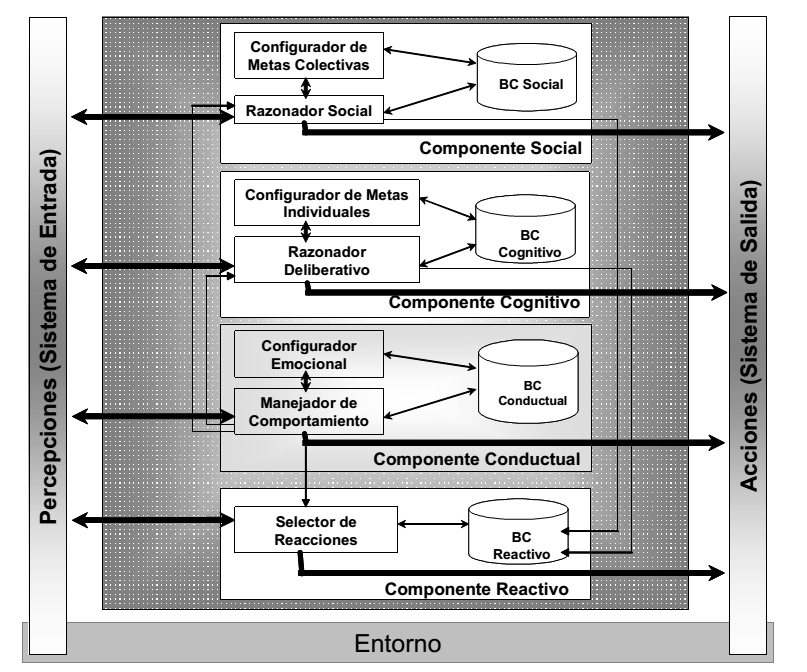
\includegraphics[width=10cm]{ilustraciones/marco-teorico/componentes-masoes-individual.jpg}
\end{ilustracion}

\subsubseccion{Modelo Emocional de MASOES}

El modelo afectivo (o emocional) propuesto por \citeauthor{perozo2011} considera un conjunto de
emociones positivas y negativas generadas desde un nivel individual o colectivo,
para de esta manera promover un comportamiento individual (Reactivo, Cognitivo)
o colectivo (Imitativo) en los agentes y así, aumentar su grado de satisfacción
y por consecuencia, el nivel de auto-organización y emergencia general en el
sistema. Este modelo afectivo está representado por un espacio bidimensional,
donde el eje $x$ representa el nivel de Activación, Excitación o Relajación del
agente (mide el grado de activación fisiológica y psicológica del agente en el
intervalo [-1, 1]), y el eje $y$ representa el nivel de satisfacción, agrado o
desagrado, también en el intervalo [-1, 1] \refpilustracion{modelo-afectivo}.

\begin{ilustracion}[fuente=\cite{perozo2011}, etiqueta=modelo-afectivo, titulo={Modelo Afectivo para MASOES}]
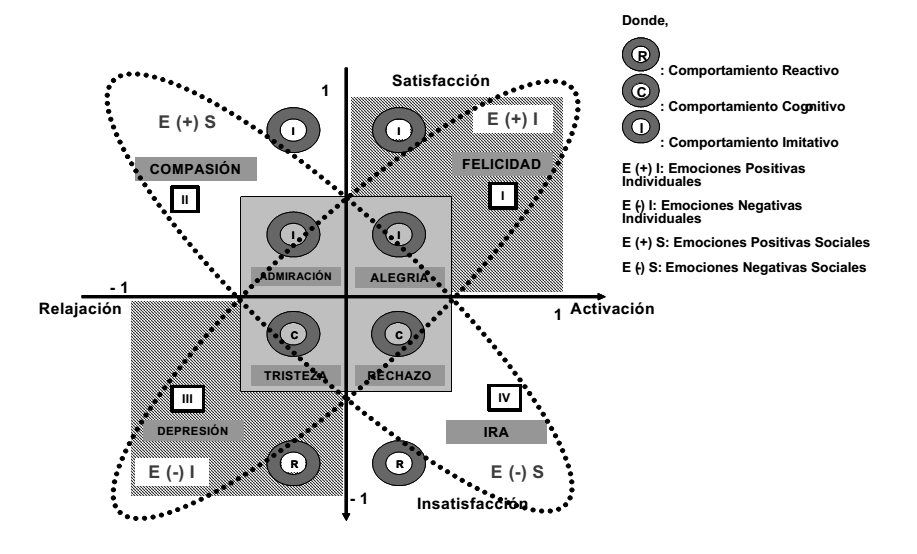
\includegraphics[width=12cm]{ilustraciones/marco-teorico/modelo-afectivo.jpg}
\end{ilustracion}

El modelo afectivo está dividido en cuatro fases:

\textbf{Fase I (Configurador Emocional):} Clasificación de las emociones. En el modelo
afectivo propuesto se consideran emociones positivas y negativas generadas desde
un nivel individual o colectivo, a fin de contribuir a la generación de un
comportamiento emergente y auto-organizado en el sistema a partir de la
interacción local de los agentes. Los tipos de emociones consideradas y el
espacio afectivo definido para MASOES, son mostrados en la \refilustracion{modelo-afectivo}. El espacio
afectivo ha sido dividido en 4 cuadrantes, donde el cuadrante I (alegría,
felicidad) y III (tristeza, depresión) representan las emociones positivas y
negativas dirigidas por la obtención de metas o logros personales (nivel
individual); y los cuadrantes II (admiración, compasión) y IV (rechazo-aversión,
ira-odio) representan las emociones positivas y negativas de tono claramente
social o interpersonal, dirigidas por las acciones de los otros agentes o
cambios en el entorno (nivel colectivo).

\textbf{Fase II (Manejador de Comportamiento):} Asociación de las emociones al tipo de
comportamiento. Para esta asociación, se le asigna a cada estado emocional del
modelo afectivo propuesto uno de los tres comportamientos considerados:
Imitativo, Cognitivo y Reactivo, de acuerdo a las reglas que se establecen \refpcuadro{comportamientos-masoes}.
Para establecer estas reglas, se considera: las emociones negativas
pueden predisponer las estrategias de resolución de problemas en los seres
humanos hacia un procesamiento local que va de lo individual a lo colectivo
(procesamiento más sistemático), mientras que las emociones positivas pueden
conducir a enfoques globales que van de lo colectivo a lo individual
(procesamiento más aproximativo).

\begin{cuadro}[etiqueta=comportamientos-masoes, titulo={Comportamientos Según el Estado Emocional del Agente}]{l|ll}
\toprule
Emoción & Tipo de Emoción & Comportamiento \\
\midrule
Felicidad & Positivo & Imitación \\
Alegría & Positivo & Imitación \\
Compasión & Positivo & Imitación \\
Admiración & Positivo & Imitación \\
Tristeza & Ligeramente Negativo & Cognitivo \\
Rechazo & Ligeramente Negativo & Cognitivo \\
Depresión & Altamente Negativo & Reactivo \\
Ira & Altamente Negativo & Reactivo \\
\bottomrule
\fuentecuadro{3}{\cite{perozo2011}}
\end{cuadro}

Por otra parte, según MASOES cada agente puede interactuar local o grupalmente.
De esta manera, si se trata de una emoción positiva el agente asumirá un
comportamiento imitativo, para llevar a cabo una acción colectiva (que va del
conocimiento colectivo al conocimiento individual) que le permita interactuar
grupalmente según los objetivos colectivos establecidos. En caso de una emoción
negativa, el agente asumirá un comportamiento reactivo o cognitivo, para llevar
a cabo una acción individual (que va del conocimiento individual al conocimiento
colectivo) que le permita interactuar localmente según los objetivos del agente
\refpilustracion{estados-comportamiento}.

\begin{ilustracion}[fuente=\cite{perozo2011}, etiqueta=estados-comportamiento, titulo={Estados Emocionales con el Tipo de Comportamiento Asociado}]
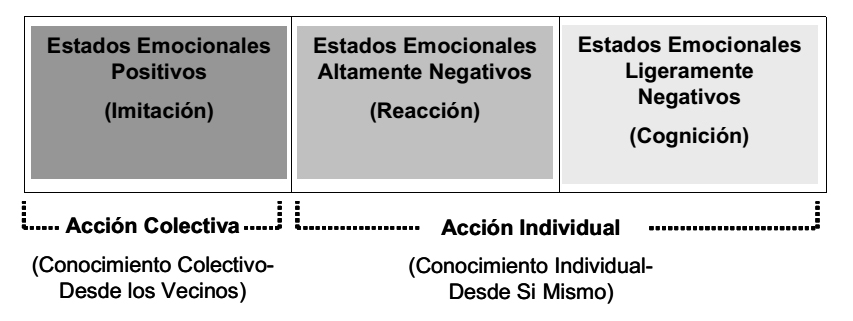
\includegraphics[width=10cm]{ilustraciones/marco-teorico/estados-comportamiento.jpg}
\end{ilustracion}

Las emociones positivas (tales como: la alegría, la felicidad, la compasión y la
admiración) conducen a un comportamiento imitativo con la idea de reproducirlo
que nos hace sentir bien a nosotros y al colectivo, mientras que las emociones
negativas (tales como: la tristeza y rechazo) nos motivan a un comportamiento
cognitivo que nos lleva a reflexionar sobre la situación actual considerando los
objetivos individuales y/o colectivos, o nos induce a un comportamiento reactivo
hacia otros en estados altamente negativo como la ira y depresión, para solo
responder de forma inmediata a la situación actual \refpcuadro{comportamientos-masoes}.
Así, para asociar los estados emocionales a un
comportamiento determinado, se tienen las siguientes reglas \refpcuadro{reglas-comportamientos-masoes}:

\newpage

\begin{cuadro}[etiqueta=reglas-comportamientos-masoes, titulo={Reglas de Priorización de Comportamientos}]{lp{7cm}}
\toprule
\textbf{Regla 1:} & Si el \textit{Estado Emocional} es \textit{Positivo} entonces priorizar \textit{Comportamiento Imitativo} \\ \hline
\textbf{Regla 2:} & Sino Si el \textit{Estado Emocional} es \textit{Ligeramente Negativo} entonces priorizar \textit{Comportamiento Cognitivo} \\  \hline
\textbf{Regla 3:} & Sino Si el \textit{Estado Emocional} es \textit{Altamente Negativo} entonces priorizar \textit{Comportamiento Reactivo} \\
\bottomrule
\fuentecuadro{2}{\cite{perozo2011}}
\end{cuadro}

\textbf{Fase III (Configurador Emocional):} Determinación de la emoción actual.

\begin{enumerate}
\item Evaluación de un evento, acción u objeto para determinar el grado de
satisfacción y activación, y luego, el estado emocional afectado. Para esta
evaluación se requiere información del mundo, tal como implicaciones de los
eventos para los agentes, los gustos o preferencias de los agentes con respecto
a objetos u otros agentes, entre otras cosas. La intensidad de la emoción
afectada viene dada por el grado de satisfacción y activación del agente, luego
de la evaluación realizada. Es necesario utilizar variables para cuantificar el
grado de satisfacción y activación del agente.
\item Modificación del actual estado emocional, si es necesario. Esta transición de
un estado a otro debe ser coherente y coordinada.
\end{enumerate}

\textbf{Fase IV (Manejador de Comportamiento):} Determinación del tipo de comportamiento.
Se modifica el comportamiento actual si es necesario, de acuerdo al estado
emocional actual y la \refcuadro{comportamientos-masoes}, como una acción resultante de la emoción
detectada en la fase anterior. De esta manera, las emociones son la expresión
dinámica y fluctuante del estado afectivo del individuo, y así, permiten cambiar
dinámicamente el tipo de comportamiento del agente de acuerdo a su situación
actual.

% \seccion{Definición de Términos Básicos}
% \hacerglosario

  	%%
% Copyright (c) {año} {nombre} <{email}>.
%
% This program is free software: you can redistribute it and/or modify
% it under the terms of the GNU General Public License as published by
% the Free Software Foundation, either version 3 of the License, or
% (at your option) any later version.
%
% This program is distributed in the hope that it will be useful,
% but WITHOUT ANY WARRANTY; without even the implied warranty of
% MERCHANTABILITY or FITNESS FOR A PARTICULAR PURPOSE.  See the
% GNU General Public License for more details.
%
% You should have received a copy of the GNU General Public License
% along with this program.  If not, see <http://www.gnu.org/licenses/>.
%%

\capitulo{Marco Metodológico}

\seccion{Tipo de Investigación}

\seccion{Población y Muestra}

\seccion{Diseño de la Investigación o Procedimiento}

\seccion{Técnicas e Instrumentos de Recolección de Datos}

\seccion{Técnicas de Procesamiento y Análisis de los Datos}

  	%%
% Copyright (c) 2017 Saúl Piña <sauljabin@gmail.com>.
%
% This program is free software: you can redistribute it and/or modify
% it under the terms of the GNU General Public License as published by
% the Free Software Foundation, either version 3 of the License, or
% (at your option) any later version.
%
% This program is distributed in the hope that it will be useful,
% but WITHOUT ANY WARRANTY; without even the implied warranty of
% MERCHANTABILITY or FITNESS FOR A PARTICULAR PURPOSE.  See the
% GNU General Public License for more details.
%
% You should have received a copy of the GNU General Public License
% along with this program.  If not, see <http://www.gnu.org/licenses/>.
%%

\capitulo{Diseño e Ingeniería de la Propuesta}

En este capítulo se describen los aspectos relacionados a la implementación
del modelo afectivo de MASOES propuesto por \cite{perozo2011}.

En primer lugar, se explican los aspectos arquitecturales de la implementación,
relevantes para entender el funcionamiento de la plataforma.
En segundo lugar, se exponen a nivel de implementación los componentes individuales y
colectivos de los agentes emocionales, descritos a nivel de diseño por \cite{perozo2011}.
Por último, se detalla lo referente a la herramienta computacional desarrollada.

\seccion{Aspectos Arquitecturales de la Propuesta}

Como paradigma de software para el desarrollo de la implementación,
se seleccionó la Programación Orientada a Agentes (POA). Este paradigma propuesto
por \cite{shoham1993agent}, esencialmente modela una aplicación como una
colección de componentes llamados agentes \citep{bellifemine2007developing}.
Permite llevar a cabo la materialización a nivel de aplicación de los sistemas
multiagente.
La POA y la Programación Orientada a Objetos (POO) son
compatibles, la primera puede ser vista como una especialización de la segunda \citep{shoham1993agent},
además, dependiendo del lenguaje de programación pueden mezclarse.

Por otra parte, se usó JADE \eningles{Java Agent
DEvelopment}, uno de los marcos de trabajo con paradigma de POA
más populares, implementado en el lenguaje de programación Java.
JADE provee bibliotecas de clases para la creación de agentes mediante
la herencia y la sobrescritura de comportamientos. Incluye
un conjunto de herramientas gráficas para la monitorización y administración de los agentes.
Además de ser un marco de trabajo, JADE se considera una plataforma,
debido a que contiene un entorno en el que los agentes se ejecutan
y se controla su ciclo de vida. Una de las caracteristica más importante de JADE
es que cumple con las especificaciones estándar FIPA \eningles{Foundation for Intelligent Physical Agents},
las cuales representan una colección de normas que tienen como objetivo promover la interoperabilidad
de agentes heterogéneos y los servicios que pueden representar. La \refilustracion{arquitectura-propuesta}
muestra la arquitectura de la plataforma JADE.

\begin{ilustracion}[fuente=\yo, etiqueta=arquitectura-propuesta, titulo={Arquitectura de JADE Conjuntamente con MASOES}]
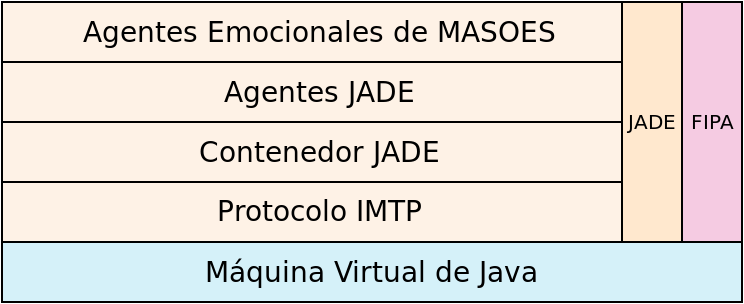
\includegraphics[width=8cm]{ilustraciones/propuesta/arquitectura.png}
\end{ilustracion}

La capa que conforma la base de la
arquitectura es la maquina virtual de Java y es la que permite
instanciar la plataforma, sobre ella se encuentra Jade, compuesta a su vez
por:

\textbf{Protocolo IMTP} \eningles{Instant Message Transfer Protocol}.
Protocolo utilizado por los agentes
para comunicarse entre sí localmente o en una red de computadores,
a través de mensajes estandarizados por FIPA \refpilustracion{comunicacion-entre-hosts}.

\textbf{Contenedor JADE}. Proporciona
todos los servicios necesarios para alojar y ejecutar agentes.

\textbf{Agentes JADE}. Son entidades de software que poseen proceso propio, comportameinto,
ciclo de vida y son capaces de recibir y enviar mensajes.

La capa superior corresponde a la implementación de los agentes emocionales
propuestos para MASOES. Dicha capa funciona como una extensión del marco de trabajo
de JADE. Proporciona un agente emocional que contiene la implementación
del componente conductual y el modelo afectivo de MASOES.

\begin{ilustracion}[fuente=\yo, etiqueta=comunicacion-entre-hosts, titulo={Comunicación Entre Agentes de JADE}]
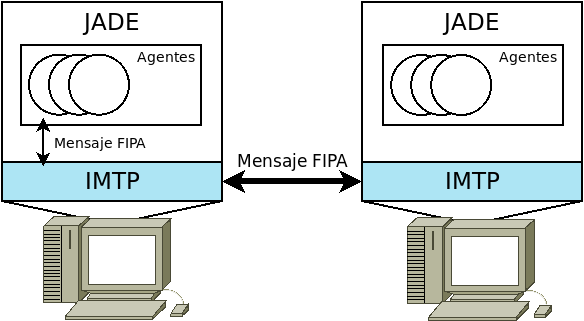
\includegraphics[width=8cm]{ilustraciones/propuesta/comunicacion-entre-hosts.png}
\end{ilustracion}

Cuando se inicia el contenedor principal, dos agentes especiales son automáticamente
instanciados por JADE, cuyos roles están definidos por FIPA y utilizan
la especificación \comillas{FIPA Agent Management} para la cuminicación a través de mensajes
\citep{fipaAgentManagement}:

\textbf{Agente AMS} \eningles{Agent Management System}. El AMS  controla la plataforma.
Es el único que puede crear y destruir a otros agentes, destruir contenedores y detener la plataforma.
Se encarga de asignarle un código a cada agente, y posee el servicio de páginas blancas, es decir,
un registro de todos los agentes. Cuando un agente desea conocer la existencia de otro
en el entorno, se comunica con el AMS.

\textbf{Agente DF} \eningles{Directory Facilitator}. El DF proporciona un directorio que
anuncia los servicios disponibles en la plataforma.
Un agente dentro del
entorno puede notificarle al agente DF cual es su rol y publicar
sus servicios (acciones), dándose a conocer a otros.

\seccion{Aspectos Propuestos a Nivel Individual}

\label{propuesta-nivel-individual}

En esta sección se describe una propuesta de ontología para MASOES
y la implementación interna de los agentes emocionales.
Además, se explica cómo ocurre el proceso de comunicación entre los agentes.

\subseccion{Propuesta de Una Ontología Para MASOES}

\label{propuesta-ontologia}

JADE requiere para la comunicación entre los agentes, la definición de una ontología.
En JADE una ontología es la definición de los conceptos y relaciones entre ellos, que forman parte
del conocimiento de un agente o una sociedad de agentes. Tanto el emisor como el receptor deben atribuir el
mismo significado a estos elementos para que la comunicación sea efectiva \citep{bellifemine2007developing}.

La necesidad de utilizar ontologías viene dada por la complejidad inherente a
las aplicaciones desarrolladas en el contexto de los sistemas multiagente, haciendo
que se presenten las siguientes dificultades: abundancia de comunicación
entre agentes, interoperabilidad de sistemas y plataformas, y problemas
semánticos.

JADE incorpora funcionalidades para codificar y decodificar las ontologías,
utilizando las especificaciones FIPA \citep{fipaOntology, fipaLanguage}.
Para construir una ontología se debe definir los siguientes elementos:

\begin{vinetas}
    \item \textit{Acciones:} son actividades que pueden llevar a cabo los agentes.
    \item \textit{Conceptos:} representan las entidades que forman parte de la ontología.
    \item \textit{Predicados:} son expresiones que relacionan los conceptos. Son
    necesarios porque en un mensaje nunca se podrá enviar directamente conceptos, solo
    predicados o acciones, los conceptos estarían encapsulados por estos dos últimos.
\end{vinetas}

Los elementos anteriormente expuestos, son proporcionados por JADE en forma de abstracciones,
de manera que puedan ser extendidas para definir una ontología de manera personalizada.
Los predicados deben heredar de \textit{Predicate},
así mismo los conceptos de \textit{Concept} y las acciones de \textit{AgentAction}. Además,
este marco de trabajo provee la clase \textit{AID} que representa el identificador único del agente,
que debe ser utilizado para asignar un emisor y receptor de un mensaje, también puede ser incluido en las
ontologías para representar a un agente.

En este trabajo se define la ontología
\comillas{\codigoenlinea{masoes}} para la
comunicación entre agentes emocionles. Dicha ontología se centra en
poder expresar dos acciones clave: evaluar un estímulo
y consultar el estado emocional.

En la \refilustracion{ontologia-masoes-estimulo} se observa las entidades que conformán la
acción evaluar estímulos.
Para solicitarle a un agente que evalúe un estímulo se le debe enviar
 una acción \textit{EvaluarEstimulo},
internamente esta contiene el concepto \textit{Estimulo} que puede ser de tres tipos,
\textit{Objeto, Accion o Evento}.
El agente en cuestión responderá con un predicado de tipo \textit{EstadoDeAgente},
el cual encapsula los conceptos \textit{EstadoDeEmocion}
y \textit{EstadoDeComportamiento}, y representa el nuevo estado emocional del agente
luego de evaluar el estímulo.
Para apreciar de mejor manera el flujo de comunicación se incluye la \refilustracion{flujo-agente-evaluar-estimulo}.

\begin{ilustracion}[fuente=\yo, etiqueta=ontologia-masoes-estimulo, titulo={Ontología para MASOES, Acción Evaluar Estímulo}]
\includegraphics[width=11cm]{ilustraciones/diagramas-puml/ontologia-masoes-estimulo.png}
\end{ilustracion}

\begin{ilustracion}[fuente=\yo, etiqueta=flujo-agente-evaluar-estimulo, titulo={Flujo de Comunicación, Acción Evaluar Estímulo}]
\includegraphics[width=11cm]{ilustraciones/diagramas-puml/flujo-agente-evaluar-estimulo.png}
\end{ilustracion}

Con respecto a la acción consultar estado emocional se tiene el diagrama de la \refilustracion{ontologia-masoes-estado}.
Es posible conocer el estado emocional de un agente enviando la acción \textit{ConsultarEstadoEmocional},
a diferencia de la acción anterior, esta no tiene ningún concepto. El agente receptor responderá
con un predicado de tipo \textit{EstadoDeAgente} y no modificará su estado emocional actual.
El flujo de comunicación se puede ver en la \refilustracion{flujo-agente-estado}.

\begin{ilustracion}[fuente=\yo, etiqueta=ontologia-masoes-estado, titulo={Ontología para MASOES, Acción Consultar Estado del Agente}]
\includegraphics[width=11cm]{ilustraciones/diagramas-puml/ontologia-masoes-estado.png}
\end{ilustracion}

\begin{ilustracion}[fuente=\yo, etiqueta=flujo-agente-estado, titulo={Flujo de Comunicación, Acción Consultar Estado del Agente}]
\includegraphics[width=8cm]{ilustraciones/diagramas-puml/flujo-agente-estado.png}
\end{ilustracion}

\subseccion{Comunicación Entre Agentes}

Los elementos más importantes en la comunicación entre agentes son:

\textbf{Acto comunicativo} o \textbf{performativa}. Definido en \cite{fipaCommnicativeAct},
se refiere al acto de comunicar en un determinado momento una acción.

\textbf{Lenguaje}. Se utilizó el lenguaje \comillas{\codigoenlinea{fipa-sl}}
\eningles{FIPA Semantic Language (SL)}, es un lenguaje estandarizado en \cite{fipaLanguage}, entendible por el humano,
ya que utiliza una codificación en texto plano.

\textbf{Protocolo}. La especificación FIPA declara diferentes protocolos para
distintas acciones o situaciones. Para el desarrollo de este trabajo se utilizó
el protocolo \comillas{\codigoenlinea{fipa-request}} definido en
\cite{fipaProtocol}. Este protocolo dicta el procedimiento que deben seguir los
agentes al recibir un mensaje y que performativas deben ser usadas para cada
acción. En la \refilustracion{flujo-fipa-protocolo-request}, se aprecia el
diagrama de secuencia de las interacciones entre el emisor y el receptor.
El emisor envía una petición al receptor (performativa
\comillas{\codigoenlinea{request}}), luego el receptor puede aceptar
(performativa \comillas{\codigoenlinea{agree}}) o rechazar la petición
(performativa \comillas{\codigoenlinea{refuse}}). En caso que el agente acepte
la petición, enviará al emisor una respuesta afirmativa (performativa
\comillas{\codigoenlinea{inform}}) si la acción se ejecutó correctamente o
fallida (performativa \comillas{\codigoenlinea{failure}}) si ocurrió un error.

\begin{ilustracion}[fuente=\cite{fipaProtocol}, etiqueta=flujo-fipa-protocolo-request, titulo={Protocolo de Petición FIPA}]
\includegraphics[width=6cm]{ilustraciones/diagramas-puml/flujo-fipa-protocolo-request.png}
\end{ilustracion}

\textbf{Ontología}. Es la definición de los conceptos y relaciones entre ellos, que forman parte
del conocimiento de un agente o una sociedad de agentes. Una ontología
es escencial para lograr una comunicación efectiva en un grupo de agentes.
Los elementos que componen una ontologia de JADE (Conceptos, Acciones y Predicados) juegan
diferentes papeles en la comunicación. Como se muestra en la \refilustracion{flujo-fipa-protocolo-ontologia},
el contenido que envía un agente emisor es de tipo \textit{AgentAction} y recibirá
como respuesta un contenido de tipo \textit{Predicate}. Los elementos de tipo \textit{Concept}
pueden ser utilizados tanto por las acciones como por los predicados, para transmitir
una información.

\begin{ilustracion}[fuente=\yo, etiqueta=flujo-fipa-protocolo-ontologia, titulo={Comunicación Entre Emisor y Receptor Usando Ontologías}]
\includegraphics[width=10cm]{ilustraciones/diagramas-puml/flujo-fipa-protocolo-ontologia.png}
\end{ilustracion}

\textbf{Mensaje ACL} \eningles{Agent Communication Language}. Es una estructura
común de transporte de información propuesta por \cite{fipaACL},
es implementada por JADE. En la \refcuadro{parametros-mensajes-acl}, se listan los parámetros
utilizados en la implementación para la comunicación entre agentes emocionales, deben ser
provistos en un mensaje para que la comunicación se logre efectuar.

\begin{cuadro}[etiqueta=parametros-mensajes-acl, titulo={Parámetros de Mensajes ACL Usados en la Implementación}]{l|l}
\toprule
 Parámetro & Descripción \\
\midrule
performative & Acto comunicativo \\
sender & Emisor \\
receiver & Receptor \\
content & Contenido del mensaje \\
conversation-id & Identificación única de la conversación \\
language & Lenguaje de codificación del contenido (\codigoenlinea{fipa-sl}) \\
ontology & Ontología del contenido (\codigoenlinea{masoes}) \\
protocol & Protocolo que rige la comunicación (\codigoenlinea{fipa-request}) \\
\bottomrule
\fuentecuadro{2}{\yo}
\end{cuadro}

\subseccion{Diseño de la Implementación a Nivel Individual}

El diseño a nivel individual de la propuesta abarca las entidades
vinculadas al agente emocional, y que permiten responder
a las solicitudes de otros agentes a traves de acciones.
La implementación se llevó a cabo de manera que pueda ser extendida o mejorada,
y para ser utilizada en sistemas multiagentes con diferentes dominios.
Uno de los aspectos relevantes de la implementación es que es no limitativa,
en otras palabras, los agentes emocionales pueden comunicarse con cualquier otro agente no emocional
o heterogéneo localmente o a través de una red de computadores e interactuar con ellos.
Por otra parte, la implementación permite que el procesamiento de un estímulo por un agente
pueda hacerse de manera individual, invocando su propio componente conductual, o
recibiendo un estimulo desde otros agentes o el entorno.
En la \refilustracion{diseno-nivel-individual}
se muestra el diseño a nivel individual de la implementación.

\begin{ilustracion}[fuente=\yo, etiqueta=diseno-nivel-individual, titulo={Diseño de la Implementación a Nivel Individual}]
\includegraphics[width=11cm]{ilustraciones/diagramas-puml/diseno-nivel-individual.png}
\end{ilustracion}

A continuación, se definen cada una de las entidades involucradas a
nivel individual:

\textbf{Agent}. Es la clase principal de JADE, todos los tipos de agentes deben
heredar de ella, e incluye otros aspectos relevantes, tales como, el envío y
recepción de mensajes, y manejo de comportamientos. Además, posee un hilo de
ejecución propio, y está bajo las especificaciones FIPA. Es la unidad básica en
la POA.

\textbf{Behaviour}. Pertenece a JADE, esta clase representa los
comportamientos, acciones, actividades o tareas que puede realizar un agente, debe
ser heredada, y sobrescrito su método \textit{action}. Un agente puede
contener uno o muchos comportamientos, y estos, pueden ser detenidos o
reanudados según la necesidad del mismo. Además, pueden ser agregados desde
otros comportamientos, o programados para ser ejecutados en momentos
específicos. Se agregan a través del método \textit{addBehaviour} de la clase
\textit{Agent}. Las implementaciones más usadas (también provistas por JADE) son:
\textit{OneShotBehaviour} (para ejecutar una acción una sola vez),
\textit{CyclicBehaviour} (para un comportamiento repetitivo) y
\textit{FSMBehaviour} (para generar un comportamiento compuesto basado en
máquinas de estado finito).

\textbf{AgenteEmocional}. Es la especialización de
la clase original \textit{Agent} de JADE, desarrollado de manera que contenga
el modelo afectivo de MASOES.
Se debe heredar de este agente en el caso de que se desee contruir un agente emocional.

\textbf{ComportamientoResponderEstado}. Esta es
una de la acciones básicas para el agente emocional, se encarga
de responder con la información del estado actual del agente a otro que
la haya solicitado. Este comportameinto se lleva a cabo cuando el
agente emocional recibe una solicitud de acción de tipo \textit{ConsultarEstadoEmocional}.

\textbf{ComportamientoEvaluarEstimulo}. Es la acción más
importante del agente emocional, debido a que es la que recibe un estímulo e
invoca las funciones del componente conductual, modificando el estado emocional
del agente. Se activa al recibir una solicitud de acción \textit{EvaluarEstimulo}.

\textbf{ComponenteConductual}. Representa el componente conductual
descrito en MASOES, encapsula el configurador emocional, el manejador de
comportamiento y la base de conocimiento conductual \refpseccion{componente-conductual}.

\textbf{EstadoDeAgente}. Clase utilizada por
\textit{ComportamientoResponderEstado} para encapsular información relacionada
al estado emocional del agente \refpseccion{propuesta-ontologia}.

\textbf{Estimulo}. Representa un objeto, evento
o acción de un agente, a ser evaluado por el configurador emocional \refpseccion{propuesta-ontologia}.

\seccion{Aspectos de la Implementación del Componente Conductual}

\label{componente-conductual}

El componente conductual es parte de la arquitectura individual del agente emocional propuesto en MASOES
\refpilustracion{componentes-masoes-individual}.
Lo constituyen la Base de Conocimiento Conductual, el Configurador Emocional y
el Manejador de Comportamiento. Favorece la adaptación de cada agente con su
entorno, ya que es el que debe establecer cual comportamiento (cognitivo, reactivo o
imitativo) tiene la prioridad más alta para responder frente a una situación.
Para esto utiliza el modelo afectivo de MASOES
\refpilustracion{modelo-afectivo}, el cual relaciona un estado emocional a un
tipo de comportamiento \refpcuadro{comportamientos-masoes}.
En escencia encapsula la implementación del Modelo Afectivo de MASOES.

\begin{ilustracion}[fuente=\yo, etiqueta=diseno-componente-conductual, titulo={Diseño de la Implementación del Componente Conductual}]
\includegraphics[width=15cm]{ilustraciones/diagramas-puml/diseno-componente-conductual.png}
\end{ilustracion}

A continuación, se definen cada una de las entidades que forman parte del
componente conductual \refpilustracion{diseno-componente-conductual}:

\textbf{BaseDeConocimientoConductual}. Contiene el conocimiento asociado con la
gestión de las emociones y comportamientos. Posee el método
\textit{agregarConocimiento} y \textit{resolverCuestionamiento}.

\textbf{EstadoEmocional}. Clase que encapsula el valor de la activación y
satisfacción del agente, además, puede convertir dichos valores
en un punto en el plano.

\textbf{ModeloAfectivo}. Es el que contiene la
implementación del modelo afectivo de MASOES \refpilustracion{modelo-afectivo},
permite obtener la emoción asociada a un estado emocional.

\textbf{ConfiguradorEmocional}. Encapsula el estado emocional actual del agente,
recibe un estímulo para realizar la actualización de la emoción a través del \textit{ModeloAfectivo}.

\textbf{ManejadorDeComportamiento}. Basándose en las reglas de selección de
comportamiento de MASOES \refpcuadro{reglas-comportamientos-masoes} y la emoción actual obtenida del configurador
emocional, puede actualizar la prioridad de comportamientos del agente
emocional.

\textbf{ComponenteConductual}. Representa el componente conductual
descrito en MASOES, encapsula el configurador emocional, el manejador de
comportamiento y la base de conocimiento conductual \refpilustracion{componentes-masoes-individual}.

\textbf{TipoDeComportamiento}. Es un enumerado que contiene los tres tipos de
comportamiento descritos en MASOES por \cite{perozo2011}: cognitivo, reactivo e imitativo.

\textbf{TipoDeEmocion}. Es un enumerado que lista los tipos de emociones
definidos en MASOES por \cite{perozo2011}: positiva,
ligeramente negativa o altamente negativa \refpcuadro{comportamientos-masoes}.

\textbf{Emocion}. Esta entidad es la representación de las emociones del modelo
afectivo de MASOES, es la clase padre de las emociones:
\textit{(Felicidad, Compasion, Ira, Alegria, Depresion, Tristeza, Admiracion y Rechazo)}.

\textbf{Geometria}. La clase geometría contiene el conjunto de puntos
que componen el polígono de la emoción en el plano \Rcuadrado.
Es de gran importancia debido a que es ella lo que verifica
si el estado emocional del agente se encuentra dentro del
polígono el cual representa.

\textbf{Punto}. Representación de un punto en el plano \Rcuadrado, utilizado por la
clase \textit{Geometria} con la finalidad de crear el polígono de la emoción.

\textbf{Estimulo}. Visto en la \refseccion{propuesta-ontologia}, contiene la información
del objeto, evento o acción que debe evaluar el componente conductual.

\subseccion{Modelo Afectivo}

Como se dijo anteriormente \refpilustracion{modelo-afectivo}, el modelo afectivo de MASOES está compuesto por 8 emociones,
distribuidas en los 4 cuadrantes del plano cartesiano, las cuales son representadas geométricamente
como polígonos regulares o irregulares.
El eje de las abscisas o $x$ representa la activación,
donde $-1 \leq x \leq 1$,
y el eje de la ordenadas o $y$ la satisfacción, donde $-1 \leq y \leq 1$.
En la implementación del modelo afectivo los puntos que conforman
los polígonos de las emociones son los siguiente:

\espaciodoble

\begin{vinetas}
\item Alegría = \{(0,0), (0,0.5), (0.5,0.5), (0.5,0)\}
\item Felicidad = \{(0,0.5), (0,1.0), (1.0,1.0), (1.0,0), (0.5,0), (0.5,0.5)\}
\item Admiración = \{(0,0), (0,0.5), (-0.5,0.5), (-0.5,0)\}
\item Compasión = \{(0,0.5), (0,1), (-1,1), (-1,0), (-0.5,0), (-0.5,0.5)\}
\item Tristeza = \{(0,0), (0,-0.5), (-0.5,-0.5), (-0.5,0)\}
\item Depresión = \{(0,-0.5), (0,-1), (-1,-1), (-1,0), (-0.5,0), (-0.5,-0.5)\}
\item Rechazo = \{(0,0), (0,-0.5), (0.5,-0.5), (0.5,0)\}
\item Ira = \{(0,-0.5), (0,-1), (1,-1), (1,0), (0.5,0), (0.5,-0.5)\}
\end{vinetas}

\begin{ilustracion}[fuente=\yo, etiqueta=modelo-afectivo-puntos, titulo={Representación Gráfica de los Puntos que Conforman los Polígonos de las Emociones}]
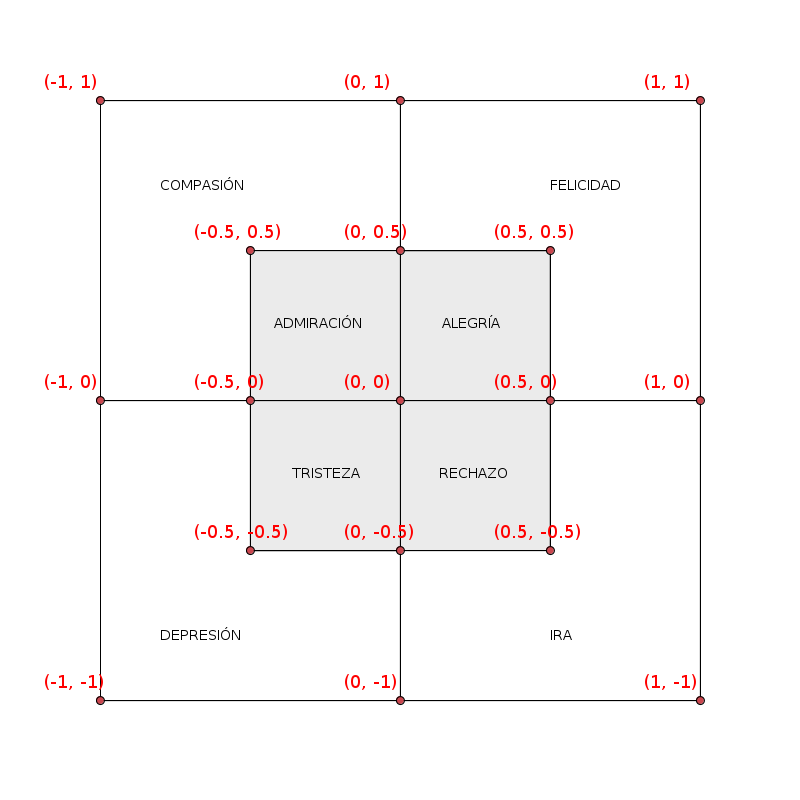
\includegraphics[width=9cm]{ilustraciones/propuesta/modelo-afectivo.png}
\end{ilustracion}

Con respecto a la selección de la emoción por parte del modelo afectivo al recibir un estado emocional,
se tiene el algoritmo de la \refcuadro{algoritmo-modelo-afectivo}, basícamente se
verifica por cada emoción si el punto en el plano proporcionado por el estado emocional
esta contenido dentro del póligono de la emoción.

\begin{cuadro}[etiqueta=algoritmo-modelo-afectivo, titulo={Algoritmo del Modelo Afectivo Para la Selección de Una Emoción}]{l}
\toprule
\textbf{Entrada:} estado emocional del agente \\
\midrule
\textbf{Para cada} emoción \textbf{$\in$} conjunto de emociones \textbf{hacer:} \\
~~~~~~\textbf{Si} el punto en \Rcuadrado~del estado emocional esta contenido \\
~~~~~~~~~~en el polígono de la emoción \textbf{entonces:} \\
~~~~~~~~~~~~~~\textbf{devolver} emoción \\
~~~~~~\textbf{Fin si} \\
\textbf{Fin para} \\
\bottomrule
\fuentecuadro{1}{\yo}
\end{cuadro}

\subseccion{Base de Conocimiento Conductual}

La Base de Conocimiento Conductual (BCC), es la responsable de la gestión del conocimiento de las
emociones y comportamientos del agente
emocional. Está implementada en el lenguaje de programación lógico \textit{Prolog},
el cual es utilizado de manera extendida para servir como base de conocimiento, debido a que
maneja hechos y reglas, además posee un motor de inferencia que permite extraer
conocimiento a través de cuestionamientos. Este lenguaje ha sido empotrado en Java
por medio del uso de bibliotecas de clases que permiten dicha asociación.

En \textit{Prolog}, un \textit{hecho} es una cláusula que representa una relación entre objetos.
Ejemplo de hecho en \textit{Prolog}: \comillas{\codigoenlinea{capital(francia, paris).}}, la interpretación es:
La capital de Francia es París. En general, la sintaxis es
\comillas{\codigoenlinea{relacion(objeto$_1$, objeto$_2$, ..., objeto$_n$).}}.
La relación se conoce como \textit{predicado} y los objetos como \textit{argumentos}.

Una \textit{regla} consta de dos partes, la cabeza y un cuerpo, ambos unidos por los
símbolos \comillas{:-}, los cuales se leen como \comillas{si} (la cabeza es verdad
si el cuerpo es verdad). La cabeza está compuesta por un solo hecho, y el cuerpo
puede estar constituido por uno o varios hechos, ejemplo:
\comillas{\codigoenlinea{cabeza :- hecho$_1$, hecho$_2$, ..., hecho$_n$.}}.
Ejemplo de regla en \textit{Prolog}: \comillas{\codigoenlinea{hijoDe(A,B) :- padrede(B,A).}},
y su interpretación es: A es hijo de B si B es padre de A.

El conocimiento gestionado por la BCC puede ser de cuatro
tipos, conocimiento sobre \textit{el agente, las emociones,
las reglas de prioridad de los comportamientos y los estímulos}.
Con respecto al agente, en la \refcuadro{conocimiento-sobre-agente}
se observan las cláusulas que definen el conocimiento
en relación a sí mismo y a los demás.

\newpage

\begin{cuadro}[etiqueta=conocimiento-sobre-agente, titulo={Conocimiento Relacionado al Agente en la BCC}]{lp{7cm}}
\toprule
Cláusula & Descripción \\
\midrule
\codigoenlinea{1. yo(agenteEmocional).} & Definición del agente actual. Se utiliza como ejemplo el nombre \codigoenlinea{agenteEmocional} \\ \hline
\codigoenlinea{2. otro(A) :- not yo(A).} & Definición de otro agente. \codigoenlinea{A} es una variable que representa el nombre del agente \\
\bottomrule
\fuentecuadro{2}{\yo}
\end{cuadro}

La \refcuadro{conocimiento-emociones}, muestra los hechos del conocimiento
asociado a los tipos de emociones. La estructura de la regla para definir
un tipo de emoción se compone del predicado, en este caso \codigoenlinea{tipo\_emocion}
y los parámetros: emoción y tipo de emoción.
Dicho conocimiento es definido por MASOES en la \refcuadro{comportamientos-masoes}.

La base de conocimiento conductual también contiene las reglas definidas
por MASOES en las que se asocia un estado emocional a un tipo de comportamiento.
Así, para las reglas de asociación de comportamiento \refpcuadro{reglas-comportamientos-masoes},
se define el conjunto de cláusulas de la
\refcuadro{conocimiento-comportamiento}, donde \codigoenlinea{E} representa la emoción.

\begin{cuadro}[etiqueta=conocimiento-emociones, titulo={Conocimiento Relacionado a las Emociones en la BCC}]{ll}
\toprule
Cláusula & Descripción \\
\midrule
\codigoenlinea{1. tipo\_emocion(admiracion, positiva).} & La admiración es positiva \\ \hline
\codigoenlinea{2. tipo\_emocion(compasion, positiva).} & La compasión es positiva \\ \hline
\codigoenlinea{3. tipo\_emocion(felicidad, positiva).} & La felicidad es positiva \\ \hline
\codigoenlinea{4. tipo\_emocion(alegria, positiva).} & La alegría es positiva \\ \hline
\codigoenlinea{5. tipo\_emocion(rechazo, ligeramente\_negativa).} & El rechazo es ligeramente negativa \\ \hline
\codigoenlinea{6. tipo\_emocion(tristeza, ligeramente\_negativa).} & La tristeza es ligeramente negativa \\ \hline
\codigoenlinea{7. tipo\_emocion(ira, altamente\_negativa).} & La ira es altamente negativa \\ \hline
\codigoenlinea{8. tipo\_emocion(depresion, altamente\_negativa).} & La depresión es altamente negativa \\
\bottomrule
\fuentecuadro{2}{\yo}
\end{cuadro}

\newpage

\begin{cuadro}[etiqueta=conocimiento-comportamiento, titulo={Conocimiento Relacionado a las Comportamientos en la BCC}]{p{6.5cm}p{5cm}}
\toprule
Cláusula & Descripción \\
\midrule
\codigoenlinea{1. prioridad\_comportamiento(E, imitativo) :- tipo\_emocion(E, positiva).} & El comportameinto es imitativo si la emoción \codigoenlinea{E} es positiva \\ \hline
\codigoenlinea{2. prioridad\_comportamiento(E, cognitivo) :- tipo\_emocion(E, ligeramente\_negativa).} & El comportameinto es cognitivo si la emoción \codigoenlinea{E} es ligeramente negativa \\ \hline
\codigoenlinea{3. prioridad\_comportamiento(E, reactivo) :- tipo\_emocion(E, altamente\_negativa).} & El comportameinto es reactivo si la emoción \codigoenlinea{E} es altamente negativa \\
\bottomrule
\fuentecuadro{2}{\yo}
\end{cuadro}

Para agregar estímulos a la BCC, es necesario que
el agente asigne a cada uno de ellos un \textit{Parámetro de Activacion ($P_a$)}
y un \textit{Parámetro de Satisfacción ($P_s$)}, estos valores
incrementarán o decrementaran la activación y satisfacción del agente.
La estructura para definir un estímulo se compone del predicado
\codigoenlinea{estimulo} y los argumentos:
nombre del agente, nombre del estímulo, $P_a$ y $P_s$.
En el \refcuadro{definicion-eventos}, se muestran algunos ejemplos de definiciones de estímulos.

\begin{cuadro}[etiqueta=definicion-eventos, titulo={Ejemplos de Conocimiento de Estímulos en la BCC}]{lp{6cm}}
\toprule
Cláusula & Descripción \\
\midrule
\codigoenlinea{1. estimulo(A, saludar, 0.01, 0.01) :- otro(A).} & Para el agente \codigoenlinea{A} el estímulo saludar aumentará la activación en 0.01 y la satisfacción en 0.01 si el estímulo fue enviado por otro agente \\ \hline
\codigoenlinea{2. estimulo(A, despertar, 0.02, -0.1) :- yo(A).} & Para el agente \codigoenlinea{A} el estímulo despertar aumentará la activación en 0.02 y disminuirá la satisfacción en 0.1 si el evento fue generado por el mismo agente \\
\bottomrule
\fuentecuadro{2}{\yo}
\end{cuadro}

\subseccion{Configurador Emocional}

Este elemento tiene la responsabilidad de evaluar los estímulos y actualizar
la emoción del agente. Para esto se definen las siguientes ecuaciones de actualización
para la activación y la satisfacción:

\begin{ecuacion}{actualizacion-activacion}
  A'(ag_i) = A_i + P_A
\end{ecuacion}

Donde $A'(ag_i)$ representa el nuevo valor de activación del agente $ag_i$,
$A_i$ es la activación actual y $P_A$ se define como el parámetro de activación
obtenido de la BCC, y esta comprendido en el intevalo: $-1 \leq P_A \leq 1$.

\begin{ecuacion}{actualizacion-satisfaccion}
  S'(ag_i) = S_i + P_S
\end{ecuacion}

Donde $S'(ag_i)$ representa el nuevo valor de satisfacción del agente $ag_i$,
$S_i$ es la satisfacción actual y $P_S$ es el parámetro de
satisfacción obtenido de la BCC, y se encuentra en el intervalo: $-1 \leq P_S \leq 1$.

Para obtener el estímulo, el configurador emocional hará un
cuestionamiento a la BCC, para ello se consulta
un hecho utilizando los símbolos \comillas{?-} con el siguiente formato en lenguaje \textit{Prolog}:

{
\ttfamily \fontsize{10pt}{10pt}\selectfont
\noindent ?- estimulo(nombreAgente, nombreEstimulo, PA, PS).
}

Las variables \comillas{\codigoenlinea{PA}} y \comillas{\codigoenlinea{PS}},
son las incógnitas a conocer.
En el siguiente ejemplo \refpcuadro{ejemplo-consulta-activacion}, se puede observar
como se consulta el evento saludar en la BCC y el formato de la respuesta de ésta.
El algoritmo de actualización del estado emocional del agente se muestra en la
\refcuadro{algoritmo-configurador-emocional}.

\newpage

\begin{cuadro}[etiqueta=ejemplo-consulta-activacion, titulo={Ejemplo de Consulta a la BCC de un Estímulo}]{ll}
\toprule
Cláusula & Descripción \\
\midrule
\codigoenlinea{1. yo(agenteA).} & Definición del agente actual \\ \hline
\codigoenlinea{2. otro(A) :- not yo(A).} & Regla que define a otros agentes \\ \hline
\codigoenlinea{3. estimulo(A, saludar, 0.01, 0.01) :- otro(A).} & Definición del estímulo saludar \\ \hline
\codigoenlinea{4. ?- estimulo(agenteB, saludar, PA, PS).} & Consulta del estímulo saludar enviado por el \codigoenlinea{agenteB} \\ \hline
\codigoenlinea{5. PA = 0.01} & Respuesta obtenida sobre el parámetro de activación \\ \hline
\codigoenlinea{6. PS = 0.01} & Respuesta obtenida sobre el parámetro de satisfacción \\
\bottomrule
\fuentecuadro{2}{\yo}
\end{cuadro}

\begin{cuadro}[etiqueta=algoritmo-configurador-emocional, titulo={Algoritmo del Configurador Emocional Para la Actualización del Estado Emocional del Agente}]{l}
\toprule
\textbf{Entrada:} estímulo y BCC \\
\midrule
Consultar en la BCC si el estímulo existe \\
\textbf{Si} existe conocimiento del estímulo \textbf{entonces:} \\
~~~~~PA  $\leftarrow$ obtener PA desde BCC \\
~~~~~PS  $\leftarrow$ obtener PS desde BCC \\
~~~~~Activación $\leftarrow$ Activación + PA \\
~~~~~Satisfacción $\leftarrow$ Satisfacción + PS \\
~~~~~Estado Emocional $\leftarrow$ Crear nuevo Estado Emocional a partir de los nuevos \\
~~~~~~~~~~~~~~~~~~~~~~~~~~~~~~~~~~~valores de Activación y Satisfacción \\
~~~~~Emoción $\leftarrow$ Consultar emoción en Modelo Afectivo a partir del nuevo Estado Emocional \\
\textbf{Fin si} \\
\bottomrule
\fuentecuadro{1}{\yo}
\end{cuadro}

\subseccion{Manejador de Comportamiento}

El Manejador de Comportamiento se encarga de actualizar la prioridad del comportamiento a ejecutar
por el agente, se basa en la reglas de prioridad definidas en MASOES \refpcuadro{reglas-comportamientos-masoes}
y el estado emocional actual.

Tiene como entrada la emoción dada por el configurador emocional.
Para obtener el tipo de comportamiento asociado a la emoción,
este componente consulta la BCC, con el siguiente formato en lenguaje \textit{Prolog}:

{
\ttfamily \fontsize{10pt}{10pt}\selectfont
\noindent ?- prioridad\_comportamiento(nombreEmocion, TIPO).
}

Este cuestionamieto retorna el valor de la variable \comillas{\codigoenlinea{TIPO}},
que puede ser \comillas{\codigoenlinea{imitativo}},
\comillas{\codigoenlinea{cognitivo}} y \comillas{\codigoenlinea{reactivo}}.

El siguiente ejemplo \refpcuadro{ejemplo-consulta-comportamiento} muestra el
resultado de preguntarle a la BCC el tipo de comportamiento asociado a la emoción
admiración.

\begin{cuadro}[etiqueta=ejemplo-consulta-comportamiento, titulo={Ejemplo de Consulta a la BCC del Tipo de Comportamiento Asociado a Una Emoción}]{p{7cm}p{5cm}}
\toprule
Cláusula & Descripción \\
\midrule
\codigoenlinea{1. tipo\_emocion(admiracion, positiva).} & Define que la Admiración es una emoción positiva \\ \hline
\codigoenlinea{2. prioridad\_comportamiento(E, imitativo) :- tipo\_emocion(E, positiva).} & Regla que define el comportameinto imitativo para una emoción \codigoenlinea{E} \\ \hline
\codigoenlinea{3. ?- prioridad\_comportamiento(admiracion, TIPO).} & Se consulta a la BCC cual es el comportamiento asociado a la admiración \\ \hline
\codigoenlinea{4. TIPO = imitativo} & Respuesta obtenida \\
\bottomrule
\fuentecuadro{2}{\yo}
\end{cuadro}

Para la actualización de la prioridad del comportamiento se implementó el algoritmo
de la \refcuadro{algoritmo-manejador-comportamiento}.

\begin{cuadro}[etiqueta=algoritmo-manejador-comportamiento, titulo={Algoritmo del Manejador de Comportamiento Para la Actualización de la Prioridad de Comportameinto}]{l}
\toprule
\textbf{Entrada:} emoción provista por el configuradoe emocional \\
\midrule
Consultar en la BCC la prioridad del comportamiento \\
\textbf{Si} existe comportamiento asociado a la emoción \textbf{entonces:} \\
~~~~~Comportamiento  $\leftarrow$ obtener comportamiento desde BCC \\
\textbf{Fin si} \\
\bottomrule
\fuentecuadro{1}{\yo}
\end{cuadro}

\subseccion{Procesamiento de Estímulo}

En el siguiente diagrama de flujo \refpilustracion{procesamiento-estimulo},
se expone el procedimiento implementado en la propuesta para realizar la gestión del estímulo
desde que se genera o recibe hasta que se actualiza el comportamiento del agente.

\begin{ilustracion}[fuente=\yo, etiqueta=procesamiento-estimulo, titulo={Flujo de Procesamiento de Estímulo}]
\includegraphics[width=12cm]{ilustraciones/diagramas-puml/procesamiento-estimulo.png}
\end{ilustracion}

El flujo puede iniciarse al recibir del entorno u otro agente un estímulo,
o al ser generado internamente, posterior a eso, el agente delega la responsabilidad a su componente
conductual, cuando el estímulo no es conocido,
el componente conductual detiene su ejecución, el flujo termina y se mantiene la emoción y comportamiento actual,
si el estímulo es conocido el componente consultará en su BCC
los parámetros de activación y satisfacción y actualizará la emoción.
Luego, el manejador de comportamiento
consulta la BCC para obtener
la prioridad asociada a la nueva emoción
que exhibe el agente, y actualiza la prioridad del comportamiento (reactivo, cognitivo o imitativo).
Finalmente, el agente modifica su comportamiento.

\seccion{Aspectos Propuestos a Nivel Colectivo}

\subseccion{Cálculo de la Emoción Social}

\cite{rincon2015} proponen un modelo de emoción social basado en el modelo
psicológico de estados emocionales PAD \eningles{Pleasure, Arousal and
Dominance}. PAD es un modelo que representa el estado emocional de un agente en
tres dimensiones, placer, excitación y dominio.
Este modelo utiliza las
emociones individuales de cada entidad de un grupo de agentes, para calcular la
\textit{emoción social}, la cual se compone de tres valores: \textit{emoción central,
distancia máxima con respecto a la emoción central y dispersión emocional}.
Basado en lo definido por \cite{rincon2015},
a continuación se expone la propuesta para el cálculo de la \textit{emoción social}:

Como está definido en MASOES \citep{perozo2011}, la emoción individual es un
vector en \Rcuadrado~y esta representada por la
\refecuacion{emocion-individual}.

\begin{ecuacion}{emocion-individual}
  E(ag_i) = (A_i , S_i)
\end{ecuacion}

Donde $ag_i$ es un agente, $A_i$ es la activación del agente y $S_i$ es la
satisfacción del agente.

La \textbf{Emoción Social} está representada por un conjunto de tres valores
\refpecuacion{emocion-social}.

\begin{ecuacion}{emocion-social}
  ES(Ag) = \{EC(Ag), m(Ag), \sigma(Ag)\}
\end{ecuacion}

Donde $Ag$ representa al grupo de agentes en estudio, $EC(Ag)$ se refiere a la
emoción central exhibida por el grupo de agentes, $m(Ag)$ es el estado emocional
más alejado de la $EC$, $\sigma(Ag)$ representa la dispersión emocional entorno
a la $EC$.

La \textbf{Emoción Central} dada por la \refecuacion{emocion-central}, se define
como la emoción promedio \refpecuacion{emocion-central-promedios} que exhibe un
grupo de agentes $Ag$, este concepto se introduce debido a que dos grupos de agentes
pueden tener la misma $EC$ para agentes muy cercanos o muy alejados de ella,
de esta manera se puede hacer una mejor interpretación de la $EC$.

\begin{ecuacion}{emocion-central}
  EC(Ag) = (\bar A(Ag), \bar S(Ag))
\end{ecuacion}

Donde $Ag$ representa al grupo de agentes en estudio, $\bar A$ es el promedio
de activación y $\bar S$ el promedio de satisfacción del grupo en estudio.

\begin{ecuacion}{emocion-central-promedios}
  \begin{split}
    \bar A(Ag)=\frac{\sum_{i=1}^n A_i}{n}, \forall ag_i \in Ag \\
    \bar S(Ag)=\frac{\sum_{i=1}^n S_i}{n}, \forall ag_i \in Ag
    \end{split}
\end{ecuacion}

Donde $Ag$ representa al grupo de agentes en estudio, $A_i$ es la activación y $S_i$ la satisfacción del agente $i$, para $1 \leq i \leq n$.

La \textbf{Distancia Máxima} con respecto a la $EC$ \refpecuacion{distancia-maxima},
permite saber si existen agentes con estados emocionales muy lejanos o cercanos
a la emoción central. Se define como la distancia máxima euclidiana
\refpecuacion{distancia-maxima-especifica} con respecto a la emoción central.

\begin{ecuacion}{distancia-maxima}
  m(Ag) = (m_A(Ag), m_S(Ag))
\end{ecuacion}

Donde $Ag$ representa al grupo de agentes en estudio, $m_A(Ag)$ es
la activación más alejada (máxima activación) y $m_S(Ag)$ es la satisfacción más
alejada (máxima satisfacción).

\begin{ecuacion}{distancia-maxima-especifica}
  \begin{split}
  m_A(Ag) = max\left(\sqrt{(A_i - \bar A(Ag))^2}\right), \forall ag_i \in Ag \\
  m_S(Ag) = max\left(\sqrt{(S_i - \bar S(Ag))^2}\right), \forall ag_i \in Ag
  \end{split}
\end{ecuacion}

Donde $Ag$ es el grupo de agentes, $A_i$ es la activación y $S_i(Ag)$ la satisfacción del agente $ag_i$,
 $\bar A$ es el promedio de activación y $\bar S(Ag)$ el promedio de satisfacción del grupo en estudio.

Para una mejor comprensión de la diversidad de emociones en el grupo de agentes,
surge la \textbf{Dispersión Emocional} entorno a la $EC$ representada por la
\refecuacion{dispersion-emocional} y se define como la desviación estándar con
respecto a la emoción central \refpecuacion{dispersion-emocional-especifica}.

\begin{ecuacion}{dispersion-emocional}
  \sigma(Ag) = (\sigma_A(Ag), \sigma_S(Ag))
\end{ecuacion}

Donde $\sigma_A(Ag)$ es la desviación estándar de la activación y
$\sigma_S(Ag)$ es la desviación estándar de la satisfacción del grupo
de agentes $Ag$.

\begin{ecuacion}{dispersion-emocional-especifica}
  \begin{split}
  \sigma_A(Ag) = \sqrt{\frac{\sum_{i=1}^n(A_i - \bar A(Ag))^2}{n}},  \forall ag_i \in Ag \\
  \sigma_S(Ag) = \sqrt{\frac{\sum_{i=1}^n(S_i - \bar S(Ag))^2}{n}},  \forall ag_i \in Ag
  \end{split}
\end{ecuacion}

Donde $Ag$ es el grupo de agentes, $A_i$ es la activación y $S_i$ la satisfacción del agente $ag_i$,
para $1 \leq i \leq n$, $\bar A(Ag)$ es el promedio de activación y $\bar S(Ag)$
el promedio de satisfacción del grupo en estudio.

Si $\sigma(Ag) \gg 0$, el grupo tiene una alta dispersión emocional, es decir, los
miembros del grupo tienen diferentes estados emocionales (muy heterogéneos).

Si $\sigma (Ag) \cong 0$, el
grupo tiene una dispersión emocional baja, esto significa que los individuos
tienen estados emocionales similares (muy homogéneos).

\seccion{Herramienta Computacional Desarrollada}

El código fuente desarrollado para este trabajo de investigación se encuentra
disponible bajo la licencia GPL \eningles{General Public License}, y se puede
acceder a través de la dirección \url{http://bit.ly/ImplementacionMASOES}.
Se utilizó \codigoenlinea{Java} como lenguaje de programación en su versión 8.

Las librerías empleadas para el desarrollo de la herramienta computacional se nombran a continuación:

\begin{vinetas}
    \item \codigoenlinea{JADE 4.4.0} como plataforma para el desarrollo de los
    agentes de software.
    \item \codigoenlinea{JTS 1.13} para los cálculos geométricos asociados al
    modelo afectivo.
    \item \codigoenlinea{Miglayout 5.0} para el desarrollo de las interfaces
    de usuario.
    \item \codigoenlinea{TuProlog 3.2} como intérprete del lenguaje Prolog dentro de Java.
    \item \codigoenlinea{jFreeChart 1.0.19} para la creación de gráficos en tiempo real.
    \item \codigoenlinea{jUnit 4.12}, \codigoenlinea{Mockito 1.10.19} y \codigoenlinea{PowerMock 1.6.5}
    en combinación para pruebas unitarias y funcionales.
    \item \codigoenlinea{commons-cli 1.3.1} como interpretador de comandos, utilizado
    en los agentes emocionales para extraer argumentos.
    \item \codigoenlinea{jackson 2.9.0} para exportar e importar una configuración a través de archivos de texto.
\end{vinetas}

\espaciodoble

La herramienta proporciona diversos comandos que permiten llevar a cabo
diferentes tareas, se listan en la \refcuadro{comandos-para-ejecuacion}:

\begin{cuadro}[etiqueta=comandos-para-ejecuacion, titulo={Lista de Comandos Para la Ejecución de la Herramienta}]{l|p{8cm}}
\toprule
Comando & Descripción \\
\midrule
\codigoenlinea{make help} & Muestra la ayuda \\
\codigoenlinea{make unit-test} & Ejecuta las pruebas unitarias \\
\codigoenlinea{make fuctional-test} & Ejecuta las pruebas funcionales \\
\codigoenlinea{make test} & Ejecuta las pruebas unitarias y funcionales a la vez \\
\codigoenlinea{make run} & Levanta la plataforma sin agentes instanciados \\
\codigoenlinea{make simulation} & Levanta la plataforma con los agentes necesarios para llevar a cabo una simulación \\
\bottomrule
\fuentecuadro{2}{\yo}
\end{cuadro}

\subseccion{Configuraciones de JADE Para la Ejecución de la Plataforma}

Se proporciona el archivo \codigoenlinea{jade.properties} en la ruta del proyecto con la finalidad
de registrar las configuraciones necesarias para la ejecución de la plataforma,
dichos valores se mustran en la \refcuadro{configuracion-jade}:

\newpage

\begin{cuadro}[etiqueta=configuracion-jade, titulo={Lista de Configuraciones de JADE Utilizadas Para la Ejecución de la Herramienta Computacional}]{l|cp{6cm}}
\toprule
Configuración & Valor por Omisión & Descripción \\
\midrule
\codigoenlinea{gui} & \codigoenlinea{true} & Le indica a JADE si la ejecución será en modo interfaz de usuario (\codigoenlinea{true}) o en modo servidor (\codigoenlinea{false}). \\
\codigoenlinea{port} & \codigoenlinea{1099} & Se refiere al puerto que utilizara JADE para conectar diferentes contenedores de agentes localmente o a través de una red. El protocolo usado es JICP \eningles{JADE Inter Container Protocol}  \\
\codigoenlinea{jade\_mtp\_http\_port} & \codigoenlinea{7778} & Puerto utilizado por JADE para la transmisión de mensajes de agentes localmente o a través de una red. El protocolo usado es IMTP \eningles{Instant Message Transfer Protocol}  \\
\codigoenlinea{jade\_domain\_df\_autocleanup} & \codigoenlinea{true} & Le indica al agente DF de JADE que debe limpiar los servicios de un agente en caso de que sea eliminado (\codigoenlinea{true}), de esta manera se asegura que no haya información inconsistente en el DF. \\
\codigoenlinea{platform-id} & \codigoenlinea{masoes} & Debido a que se puede instanciar diferentes plataformas localmente o en una red, es necesario asignar un identificador único a cada una. \\
\bottomrule
\fuentecuadro{3}{\yo}
\end{cuadro}

\subseccion{Agentes del Entorno Propuestos Para MASOES}

El entorno está constituido por diversos agentes emocionales y no emocionales,
con la finalidad de cumplir diversos roles necesarios para el funcionamiento de
la implementación, por esta razón se proponen los siguientes agentes.

\subsubseccion{Agente Emocional}

En la \refseccion{propuesta-nivel-individual} se vió el diseño del agente emocional a nivel individual.
A continuación se listan los argumentos (opcionales) que pueden ser enviados al agente al momento de ser
instanciado en la plataforma:

\begin{cuadro}[etiqueta=argumentos-agente-emocional, titulo={Lista de Argumentos Para el Agente Emocional}]{l|p{8cm}}
\toprule
Argumento & Descripción \\
\midrule
\codigoenlinea{a} & \textbf{Activación:} Asigna la activación inicial del agente emocional \\
\codigoenlinea{s} & \textbf{Satisfacción:} Asigna la satisfacción inicial del agente emocional\\
\codigoenlinea{k} & \textbf{Importar Conocimiento:} Permite importar al agente conocimiento desde una cadena de caracteres \\
\codigoenlinea{kp} & \textbf{Importar Conocimiento Desde Archivo de Texto:} Ruta del archivo de texto con el conocimiento sobre los estímulos para el agente \\
\bottomrule
\fuentecuadro{2}{\yo}
\end{cuadro}

\subsubseccion{Agente Notificador}

El Agente Notificador tiene como responsabilidad notificar a todos los agentes de
las acciones, objetos o eventos que van aconteciendo en el sistema.
Se desarrolló para este trabajo de investigación con el objetivo de comunicar una
acción, objeto o evento al resto de agentes del campo de acción.

En la \refilustracion{ontologia-masoes-notificar-estimulo},
se observan las entidades de la ontología propuesta para MASOES, que permiten la interacción
con este agente. Cualquier agente puede enviar una notificación de tipo objeto, acción o evento,
cuando la acción se haya completado el agente notificador enviará una respuesta tipo \textit{Done},
esta entidad es provista por JADE e indica que la solicitud fue realizada satisfactoriamente.

\begin{ilustracion}[fuente=\yo, etiqueta=ontologia-masoes-notificar-estimulo, titulo={Ontología para MASOES, Acciones de Notificación}]
\includegraphics[width=11cm]{ilustraciones/diagramas-puml/ontologia-masoes-notificar-estimulo.png}
\end{ilustracion}

A través del diagrama de la \refilustracion{flujo-agente-notificador}, se explica el procedimiento
que realiza este agente para comunicar un estímulo. En primer lugar, recibe una petición de acción,
luego solicita la lista de agentes emocionales al DF, por último, envía un estímulo
a cada agente de la lista y responde con un objeto \textit{Done} al agente emisor.

\begin{ilustracion}[fuente=\yo, etiqueta=flujo-agente-notificador, titulo={Comunicación con el Agente Notificador}]
\includegraphics[width=11cm]{ilustraciones/diagramas-puml/flujo-agente-notificador.png}
\end{ilustracion}

\subsubseccion{Agente Para el Cálculo de la Emoción Social}

\label{agente-calculador-emocion-social}

Se propone un agente
que encapsula el cálculo de la emoción social
propuesta en este trabajo. Se incluyen entidades en la ontología de MASOES que permiten
la interacción con otros agentes.
Para que un agente pueda conocer la emoción social
debe enviar una solicitud de tipo \textit{ConsultarEmocionSocial},
el agente calculador enviará una respuesta de tipo \textit{EmocionSocial}
con los valores de la emoción central, dispersión emocional
y distancia máxima \refpilustracion{ontologia-masoes-emocion-social}.

En el diagrama de la \refilustracion{flujo-agente-emocion-social}, se ilustra el procedimiento
de comunicación entre agentes, se incluye las entidades ontológicas usadas en dicha comunicación.
Este agente debe consultar al DF el listado de agentes emocionales en la plataforma,
posteriormente, solicita el estado emocional a cada uno de ellos y procede a calcular la emoción
social.

\begin{ilustracion}[fuente=\yo, etiqueta=ontologia-masoes-emocion-social, titulo={Ontología para MASOES, Acción Consultar Emoción Social}]
\includegraphics[width=12cm]{ilustraciones/diagramas-puml/ontologia-masoes-emocion-social.png}
\end{ilustracion}

\begin{ilustracion}[fuente=\yo, etiqueta=flujo-agente-emocion-social, titulo={Comunicación con el Agente Calculador de Emoción Social}]
\includegraphics[width=13cm]{ilustraciones/diagramas-puml/flujo-agente-emocion-social.png}
\end{ilustracion}

\subsubseccion{Agente Interfaz: Estado del Agente}

Es posible observar el estado emocional de un agente en tiempo de ejecución a través de la interfaz
\comillas{Estado del Agente} \refpilustracion{interfaz-estado-agente}.
Esta incluye el gráfico del modelo afectivo de MASOES y la información correspondiente al estado emocional.
Se debe crear en la plataforma un agente de tipo: \codigoenlinea{gui.agentstate.AgentStateGuiAgent},
dandole como argumento el
nombre del agente el cual se desea observar su estado emocional.

\begin{ilustracion}[fuente=\yo, etiqueta=interfaz-estado-agente, titulo={Interfaz Para Observar el Estado Emocional Dado un Agente}]
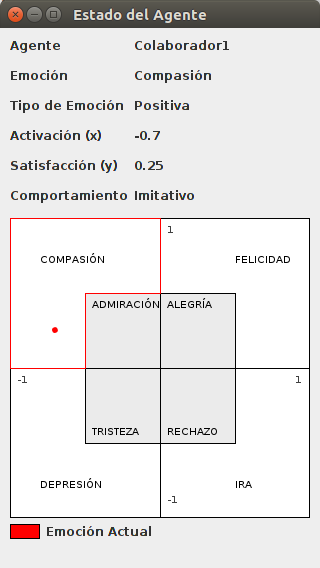
\includegraphics[width=7cm]{ilustraciones/interfaces/estado-agente.png}
\end{ilustracion}

\subsubseccion{Agente Interfaz: Emoción Social}

Se proporciona la interfaz \comillas{Emoción Social} para poder observar la emoción social actual
en tiempo de ejecución \refpilustracion{interfaz-emocion-social}, dicha interfaz se conectara automáticamente con el agente descrito en la \refseccion{agente-calculador-emocion-social}.
Esta incluye el gráfico del modelo afectivo de MASOES y la información correspondiente a
la emoción social. Se debe instanciar en la plataforma un agente de tipo: \codigoenlinea{gui.socialemotion.SocialEmotionGuiAgent}.

\begin{ilustracion}[fuente=\yo, etiqueta=interfaz-emocion-social, titulo={Interfaz Para Observar la Emoción Social del Grupo de Agentes}]
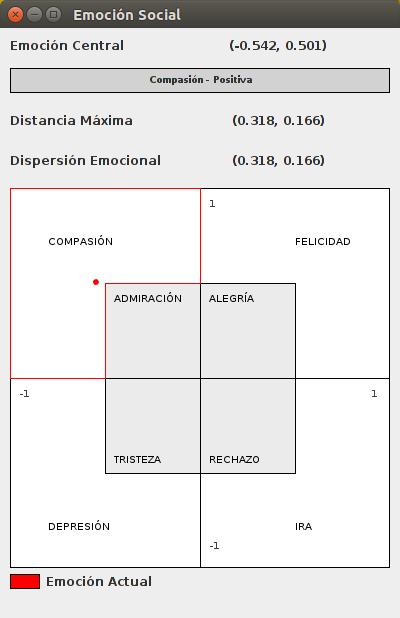
\includegraphics[width=8cm]{ilustraciones/interfaces/emocion-social.png}
\end{ilustracion}

\subsubseccion{Agente Interfaz: Para el Envío de Mensajes}

En la \refilustracion{envio-de-mensajes}
se muestra la ventana para envío de mensajes manualmente, es desarrollada con la finalidad de observar
los mensajes que se envían y reciben en una conversación entre dos agentes.
Se instancia a través de la clase: \codigoenlinea{gui.requester.RequesterGuiAgent}.

\begin{ilustracion}[fuente=\yo, etiqueta=envio-de-mensajes, titulo={Interfaz Para Envío de Mensajes Manualmente}]
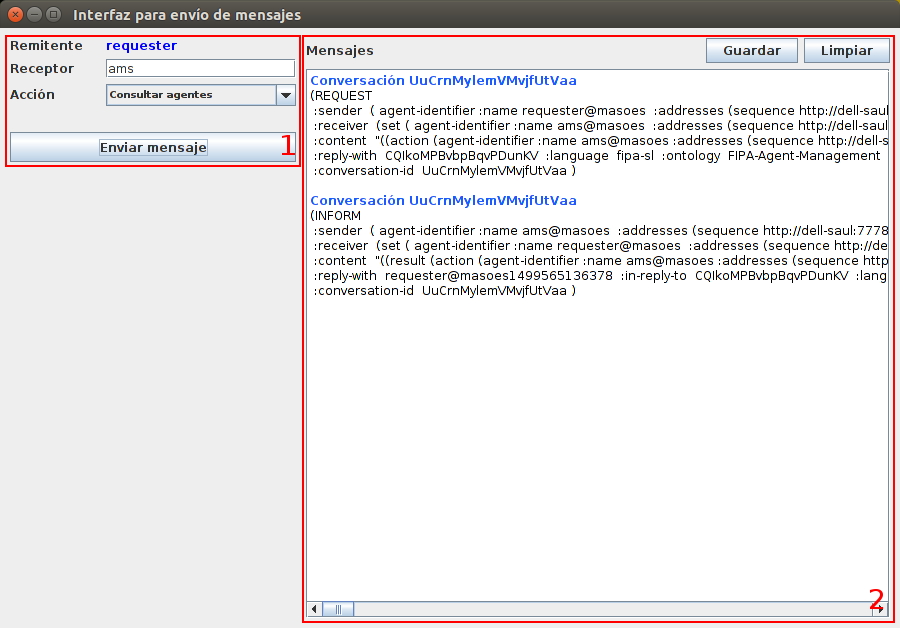
\includegraphics[width=14cm]{ilustraciones/interfaces/interfaz-para-envio-de-mensajes-recuadros.png}
\end{ilustracion}

Dicha interfaz se compone de dos secciones:

\begin{enumeracion}
	\item \textbf{Acciones:} Permite configurar el mensaje que se enviará, contiene un conjunto de mensajes o acciones
  preconfiguradas.
	\item \textbf{Mensajes}: Muestra los mensajes enviados y recibidos, además, proporciona dos botones
  que permiten guardar los mensajes en un archivo de texto y limpiar la ventana.
\end{enumeracion}

\subsubseccion{Agente Interfaz: Simulador}

La interfaz de usuario denominada simulador \refpilustracion{simulador},
permite definir los tipos de agentes y estímulos para un determinado caso de estudio, además
provee la posibilidad de establecer una configuración inicial para cada agente
(como el estado emocional y estímulos asociados a dicho agente) e instancia los agentes en la plataforma.

\begin{ilustracion}[fuente=\yo, etiqueta=simulador, titulo={Interfaz Para la Configuración de Simulaciones}]
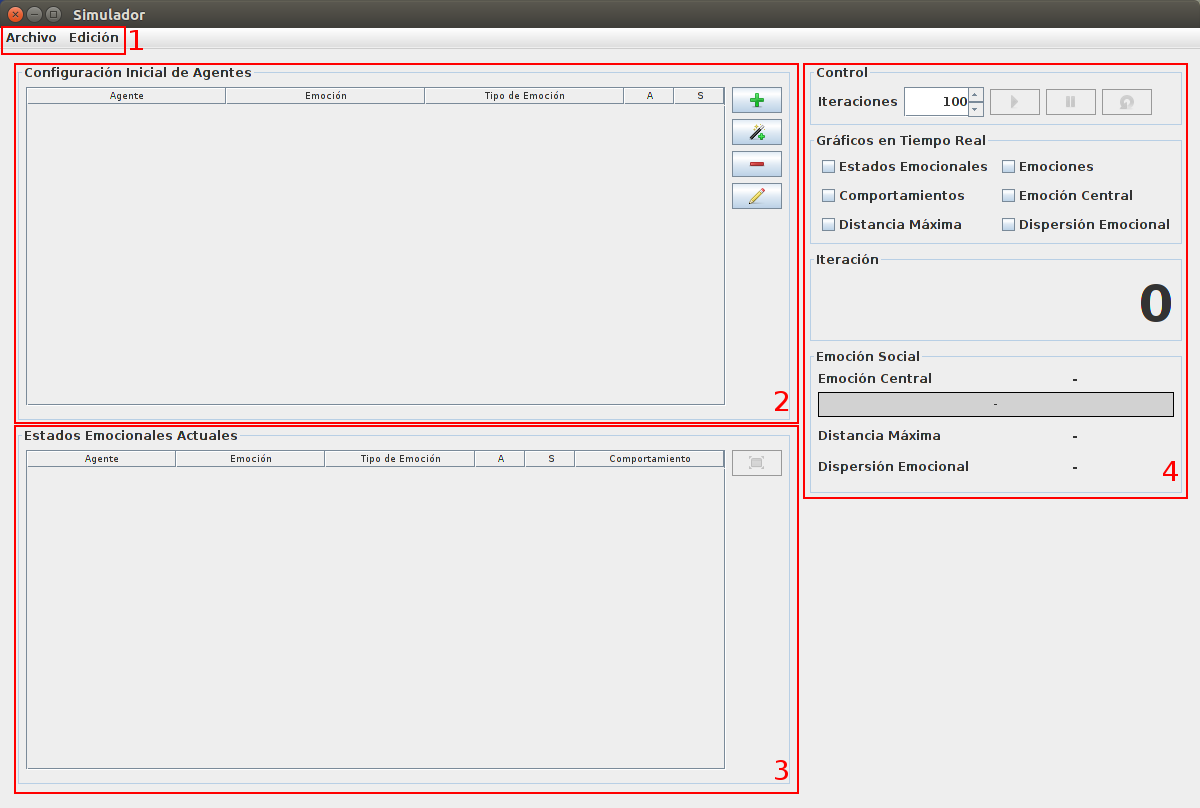
\includegraphics[width=14cm]{ilustraciones/interfaces/simulador-recuadros.png}
\end{ilustracion}

Las secciones que la componen son:

\begin{enumeracion}
	\item \textbf{Barra de Menú:} En el menú \textit{Archivo} se proveen las opciones exportar e importar configuración.
  A traves del menú \textit{Edición} se pueden definir los tipos de agentes y estímulos necesarios para la simulación.
  \item \textbf{Configuración Inicial de Agentes:} permite establecer los parámetres de cada agente en la simulación.
  \item \textbf{Estados Emocionales Actuales:} esta tabla muestra los estados emocionales del grupo de agentes en tiempo de ejecución de la simulación.
  \item \textbf{Información General de la Simulación:} en esta sección se puede controlar la simulación,
  activar o desactivar gráficos en tiempo real, asignar el número de iteraciones deseados y ver la iteración y
  la emoción social actual.
\end{enumeracion}

\subseccion{Servicios Expuestos en Agente DF}

Para que los agentes dentro de la plataforma JADE descubran
las acciones que pueden llevar a cabo los demás, se publican los siguientes servicios \refpcuadro{servicios-df}.
Cada agente al ser creado en JADE notificará sus servicios al DF,
es importante destacar que dichos servicios concuerdan con las acciones
en la ontología propuesta para MASOES.

\begin{cuadro}[etiqueta=servicios-df, titulo={Lista de Servicios Expuestos en el Agente DF para la Ontología Propuesta para MASOES}]{l|l}
\toprule
Agente & Servicio \\
\midrule
Agente Emocional & \textit{EvaluarEstimulo} \\
& \textit{ConsultarEstadoEmocional} \\
Agente Notificador  & \textit{NotificarObjeto} \\
& \textit{NotificarAccion} \\
& \textit{NotificarEvento} \\
Agente Calculador de Emoción Social & \textit{ConsultarEmocionSocial} \\
\bottomrule
\fuentecuadro{2}{\yo}
\end{cuadro}

  	%%
% Copyright (c) 2017 Saúl Piña <sauljabin@gmail.com>.
%
% This program is free software: you can redistribute it and/or modify
% it under the terms of the GNU General Public License as published by
% the Free Software Foundation, either version 3 of the License, or
% (at your option) any later version.
%
% This program is distributed in the hope that it will be useful,
% but WITHOUT ANY WARRANTY; without even the implied warranty of
% MERCHANTABILITY or FITNESS FOR A PARTICULAR PURPOSE.  See the
% GNU General Public License for more details.
%
% You should have received a copy of the GNU General Public License
% along with this program.  If not, see <http://www.gnu.org/licenses/>.
%%

\capitulo{Casos de Estudio}

En este capítulo se presentan los casos de estudio realizados, a fin de verificar que
la implementación del modelo afectivo de MASOES genere correctamente
emociones a nivel individual y colectivo.
Se utilizaron como base de comparación los
resultados obtenidos a nivel de diseño por \cite{perozo2012}, en el caso de
estudio Wikipedia.

Wikipedia es una enciclopedia de contenido libre que todos pueden editar. Esta
enciclopedia es el resultado de un trabajo colectivo, donde cada artículo es el
producto de múltiples contribuciones, que son mejoras y extensiones de un
borrador inicial \citep{perozo2011}.
Es posible gracias al esfuerzo de colaboradores en todo el
mundo, que de forma voluntaria contribuyen con artículos
y construyen una reputación en la comunidad.
La reputación de un colaborador incrementará a medida que realice
aportes a la comunidad, y disminuirá cuando dichos aportes sean editados por
otros, en otras palabras, un colaborador gana reputación cuando
sus aportes son preservados en el tiempo, y pierde reputación cuando su trabajo
va desapareciendo debido a las ediciones de otros wikipedistas.
Diferentes investigaciones sobre la reputación
y confiabilidad en Wikipedia \citep{anthony2009reputation, javanmardi2009user,
de2011reputation}, concuerdan que no solo los usuarios con mayor reputación son
los más propensos a colaborar, sino que también generan contenido de mejor
calidad.

En el modelo realizado por \cite{perozo2011}
se expone un conjunto de agentes que cumplen diversos roles y tareas de manera individual o colectiva.
Los wikipedistas (agentes) interactúan en un espacio común (entorno web) usando el mismo
editor y obedeciendo el mismo conjunto de reglas.
Dicho conjunto de agentes se describen a continuación \refpcuadro{actores-wikipedia}:

\begin{cuadro}[etiqueta=actores-wikipedia, titulo={Actores con Algunas de sus Tareas en Wikipedia}]{p{2cm}|p{5cm}p{6cm}}
\toprule
Actor & Descripción & Tareas \\
\midrule
Desarrollador
& Es un agente implicado en el mantenimiento de los servidores y/o el desarrollo
del software de Wikipedia. Además, ellos conceden los privilegios del sistema a los administradores y burócratas.
& Crear portales sobre tópicos específicos. Desarrollar código para mejorar MediaWiki.
Hacer páginas de documentación o tutoriales. Crear plantillas y algoritmos.
Mantener los Servidores. Conceder privilegios a administradores y burócratas.
Bloquear y desbloquear IP's. Participar en la votación por candidatos a artículos
sobresalientes, país de la semana y administrador.  \\ \hline

Burócrata
& Es una clase especial de administrador que es capaz de nombrar o
eliminar a otros administradores y burócratas. La existencia de los burócratas
es para aliviar las tareas de los desarrolladores.
& Nombrar y eliminar a otros burócratas y operadores del sistema. \\ \hline

Administrador
& Estos agentes poseen las mismas responsabilidades que los agentes burócratas,
y son, además, capaces de cambiar el rol de cualquier agente dado. Además,
ellos son los últimos árbitros en cualquier conflicto de Wikipedia
& Nombrar y eliminar a otros administradores, operadores del sistema y burócratas.
Arbitrar en conflictos serios, sobre la gestión de contenido en Wikipedia. \\ \hline

Operador del Sistema o Sysop \eningles{System Operator}
& Es un wikipedista que puede acceder a algunas funciones restringidas del software de Wikipedia.
Casi todos los poderes de estos administradores son completamente reversibles por cualquier
otro sysop (incluyendo la supresión y bloqueo de las direcciones IP) u operador del sistema.
& Borrar páginas e imágenes. Ver y recuperar páginas borradas e imágenes. Bloquear y
desbloquear IP de usuarios anónimos. Bloquear y desbloquear a usuarios registrados.
Proteger o bloquear una página así como las funciones inversas. Editar en páginas
protegidas o bloqueadas. Revertir páginas rápidamente. Editar el espacio de nombres de MediaWiki.
Mediar conflictos. Cerrar debates para borrado. Combatir el vandalismo.
Participar en la votación por candidatos a artículos sobresalientes, país de la semana
y operadores del sistema. \\ \hline

Usuario Registrado
& Es un agente que ha creado su nombre de usuario con su contraseña.
Puede tener una lista con sus contribuciones.
También, puede tener una página con información personal,
facilitar un correo electrónico de contacto, y tener \comillas{una página de discusión}
desde donde otros usuarios pueden comentarle cosas o establecer diálogos.
Las contribuciones de un usuario registrado son identificadas con su apodo \eningles{Nickname} en el archivo histórico de artículos.
& Adquirir experiencia en el empleo de técnicas para la sintaxis y edición de artículos. Mantener su página personal.
Interactuar recíprocamente con otros usuarios a través de su página de discusión.
Personalizar los aspectos de apariencia de la Wikipedia y el ambiente de edición de artículos.
Vigilar ciertos artículos (incorporados a su propia lista de seguimiento) para comprobar los
cambios introducidos en ellos y participar cuando él lo considere necesario.
Transferir un artículo (necesario para fusionar páginas). Editar página de discusión o artículo.
Solicitar borrado de artículo. Combatir el vandalismo. Demostrar su buena fe, haciendo contribuciones
útiles durante un tiempo. Participar en la votación por candidatos a artículos sobresalientes, país de
la semana y operadores del sistema. Verificar derechos de autor. \\ \hline

Usuario \comillas{Bot}
& Estos agentes son como \comillas{robots de software} que funcionan tanto autónomamente como manualmente para hacer tareas repetitivas.
Además, son usuarios que han sido creados por cualquier usuario registrado o administrativo en Wikipedia.
& Actualizar y mejorar las páginas por tópicos para reducir los enlaces redundantes.
Creación de nuevas páginas basadas en información ya desarrollada, y revisión de ortografía. \\ \hline

Usuario Anónimo
& Estos agentes no se han registrado en el sistema con un nombre de usuario y una contraseña.
Pueden editar casi cualquier artículo o página de discusión pero no tiene algunas funcionalidades.
Sus intervenciones son identificadas en el archivo histórico del artículo por su IP de acceso.
& Adquirir experiencia en el empleo de técnicas para la sintaxis y edición de artículos.
Editar página de discusión o artículo. Solicitar borrado de artículo. Combatir vandalismo.
Verificar Derechos de autor. \\
\bottomrule
\fuentecuadro{3}{\cite{perozo2011}}
\end{cuadro}

Para llevar a cabo los casos de estudio se selecciona como agente al \textit{Usuario Registrado},
debido a que es el actor que concentra la mayoría de contribuciones en Wikipedia.
Además, se proponen los estímulos de la \refcuadro{estimulos-propuestos}, estos
se basan en las tareas y responsabilidades que se asocian a la reputación de dicho agente.  A cada estímulo
se le asigna un valor de $P_a$ y $P_s$ según el impacto previsto sobre el agente.

\begin{cuadro}[etiqueta=estimulos-propuestos, titulo={Estímulos Asociados al Usuario Registrado Propuestos para los Casos de Estudio de Wikipedia}]{p{4cm}|rrp{7cm}}
\toprule
Estímulo & $P_a$ & $P_s$ & Descripción \\
\midrule
\multicolumn{4}{l}{\textbf{Aumento de Reputación}} \\ \hline
Artículo Nuevo & 0.05 & 0.05 & Es un estímulo que desencadena una emoción positiva, debido a que los aportes realizados son valorados por la comunidad, favoreciendo un comportamiento imitativo \\ \hline
Nueva Edición & 0.03 & 0.04 & Los agentes que más previenen el vandalismo son los usuarios registrados, las nuevas ediciones en artículos de la comunidad pueden estimular un comportamiento imitativo en este agente para que se mantenga revisando y aportando contribuciones \\ \hline
Artículo Sobresaliente & 0.08 & 0.08 & Es un mecanismo para motivar y premiar las contribuciones sobresalientes de los Wikipedistas, por ende este estímulo incrementaría de gran manera la activación y la satisfacción del agente \\ \hline
\multicolumn{4}{l}{\textbf{Decremento de Reputación}} \\ \hline
Guerra de Ediciones & -0.08 & -0.08 & Una Guerra de ediciones es definida por Wikipedia como 3 ediciones de
texto por un usuario particular en un artículo dado dentro de 24 horas, entre
las ediciones de otros usuarios. Participar en una guerra de ediciones puede hacer que este agente exhiba emociones negativas \\ \hline
Artículo Borrado & -0.06 & -0.06 & Este estímulo favorece las emociones negativas, ya que, este agente puede experimentar desánimo al sentir que su trabajo ha sido en vano  \\ \hline
Artículo Modificado & -0.02 & -0.03 & Cuando un artículo propuesto es editado por otros puede hacer que este agente experimente una disminución de su satisfacción debido a que su contribución no fue tan buena \\
\bottomrule
\fuentecuadro{4}{\yo}
\end{cuadro}

\seccion{Caso de Estudio 1: Emociones a Nivel Social}

El objetivo para este caso de estudio es verificar la correcta generación de la
Emoción Social ($ES(Ag)$) de un grupo de agentes
e interpretar los resultados obtenidos sobre la Emoción Central ($EC(Ag)$), Distancia Máxima ($m(Ag)$) y
Dispersión Emocional ($\sigma(Ag)$).
Para ello se plantean escenarios con baja dispersión emocional (agentes con emociones muy homogéneas)
y alta dispersión emocional (agentes con emociones muy heterogéneas).

Los valores obtenidos de la emoción social son muy importantes, ya que, con ellos
se puede describir el estado emocional colectivo de un grupo de agentes emocionales.
Aunque la emoción central
puede dar una idea sobre en que cuadrante del modelo afectivo se conglomeran la mayor cantidad de agentes,
son la distancia máxima y la dispersión emocional las que ayudan a determinar realmente la variación entre los diferentes estados emocionales
existentes en un grupo de agentes.
Es importante resaltar la diferencia entre dispersión emocional y distancia máxima, aunque ambas utilizan la emoción central
como base de cálculo, el objetivo de la primera es expresar la variación entre los diferentes estados emocionales presentes en un grupo de agentes
y la segunda busca identificar el estado emocional más alejado del grupo.

\subseccion{Escenario 1: Baja Dispersión Emocional y Bajo Número de Agentes}

Con la finalidad de observar y de verificar el cálculo de la emoción social,
se acota la simulación de este escenario a 10
iteraciones y a la instanciación de 3 agentes de tipo Usuario Registrado.
Estos agentes son inicializados con la emoción Alegría (ver \refcuadro{resultadoscaso1escenario1}, iteración 0).
En cada iteración se selecciona aleatoriamente un estímulo para ser enviado a cada agente.
En la \refcuadro{resultadoscaso1escenario1}, se presenta la evolución y el resultado final de la $ES(Ag)$,
por cada iteración se muestra el estímulo enviado a cada uno de los
agentes, el estado emocional (Activación \comillas{A} y Satisfacción \comillas{S}),
emoción y comportamiento que dio como resultado. Además, se incluyen por iteración los valores de la Emoción Social
(Emoción Central \comillas{$EC(Ag)$}, Distancia Máxima \comillas{$m(Ag)$} y
Dispersión Emocional \comillas{$\sigma(Ag)$}) .

Para este escenario, se supone que los Usuarios Registrados reciben solo estímulos
positivos que pueden aumentar su reputación \refpcuadro{estimulos-propuestos},
los usuarios podrían experimentar un alto grado de satisfacción y activación, que se traduciría
en emociones positivas individuales (Felicidad), lo que conllevaría a un comportamiento imitativo,
de acuerdo al modelo afectivo de MASOES. Con respecto a la emoción social, también se
vería afectada de manera positiva a la par con los agentes emocionales,
además, según lo propuesto en este trabajo, el cálculo de la dispersión
emocional ($\sigma(Ag)$) del grupo de agentes debe ser cercano a cero, debido a que los estados
emocionales de estos se encontrarían muy próximos entre sí.

En este caso, la $EC(Ag)$ fue igual a: $(0.737, 0.763)$ que corresponde a la emoción Felicidad \refpilustracion{emocion-central-final-caso1escenario1},
con una $\sigma(Ag)$ con valores muy cercanos
a cero, tanto para la activación como para la satisfacción: $(0.077, 0.078)$,
en otras palabras, el grupo de agentes exhibe emociones muy homogéneas.
También, la $m(Ag)$ expresa que los estados emocionales
de los agentes se encuentran muy cercanos: $(0.107, 0.103)$.
Asimismo, la \refcuadro{resultadoscaso1escenario1} muestra un incremento
gradual en la satisfacción y activación de los agentes, pasando de la
Alegría a la Felicidad, igualmente para la $EC(Ag)$. Por otra parte, se observa que la
dispersión emocional tuvo poca variación \refpilustracion{dispersion-emocional-final-caso1escenario1}
durante la simulación.
Los resultados obtenidos evidencian que para un grupo
de agentes con estados emocionales muy cercanos, el cálculo de la $ES(Ag)$
cumple con lo propuesto en este trabajo.

\begin{ilustracion}[fuente=\yo, etiqueta=emocion-central-final-caso1escenario1, titulo={Emoción Central Final ($EC(Ag)$), Caso de Estudio 1 Escenario 1}]
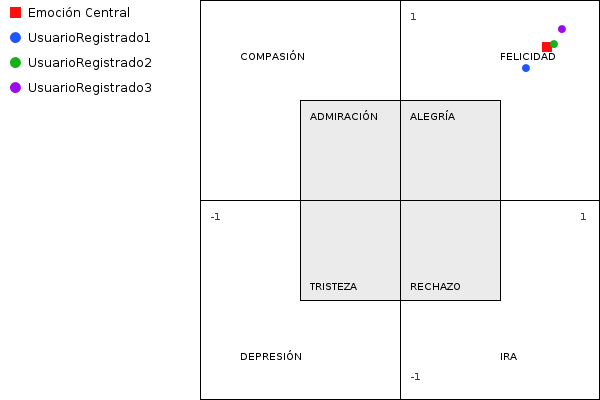
\includegraphics[width=11cm]{ilustraciones/resultados/caso1escenario1-emocioncentral.png}
\end{ilustracion}

\begin{ilustracion}[fuente=\yo, etiqueta=dispersion-emocional-final-caso1escenario1, titulo={Evolución de la Dispersión Emocional ($\sigma(Ag)$), Caso de Estudio 1 Escenario 1}]
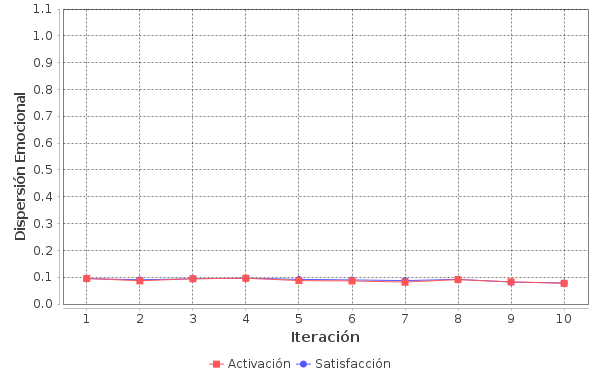
\includegraphics[width=11cm]{ilustraciones/resultados/caso1escenario1-dispersionemocional.png}
\end{ilustracion}

\clearpage
\newpage

\begin{sidewaysfigure}

\begin{cuadro}[etiqueta=resultadoscaso1escenario1, titulo={Evolución de la Emoción Social del Grupo de Agentes ($Ag$), Caso de Estudio 1 Escenario 1}, letra=\tiny]{c|l|l|c|c|l|l|c|c|l|c|c|c|c}
\toprule
\multirow{2}{*}{\textbf{Iteración}} & \multicolumn{6}{c|}{\textbf{Agentes}} &  \multicolumn{3}{c|}{\textbf{$EC(Ag)$}} & \multicolumn{2}{c|}{\textbf{$m(Ag)$}} & \multicolumn{2}{c}{\textbf{$\sigma(Ag)$}} \\ \cline{2-14}
& Nombre & Estímulo & A & S & Emoción & Comportamiento & A & S & Emoción & A & S & A & S \\
\midrule[1pt]
\multirow{3}{*}{0} & UsuarioRegistrado1 & & 0.1 & 0.1 & Alegría & Imitativo & \multirow{3}{*}{0.2} & \multirow{3}{*}{0.2} & \multirow{3}{*}{Alegría} & \multirow{3}{*}{0.1} & \multirow{3}{*}{0.1} & \multirow{3}{*}{0.082} & \multirow{3}{*}{0.082}  \\\cline{2-7}
& UsuarioRegistrado2 & & 0.2 & 0.2 & Alegría & Imitativo & & & & & & & \\ \cline{2-7}
& UsuarioRegistrado3 & & 0.3 & 0.3 & Alegría & Imitativo & & & & & & & \\ \midrule[1pt]
\multirow{3}{*}{1} & UsuarioRegistrado1 & Artículo Nuevo & 0.15 & 0.15 & Alegría & Imitativo & \multirow{3}{*}{0.253} & \multirow{3}{*}{0.257} & \multirow{3}{*}{Alegría} & \multirow{3}{*}{0.127} & \multirow{3}{*}{0.123} & \multirow{3}{*}{0.095} & \multirow{3}{*}{0.095}  \\\cline{2-7}
& UsuarioRegistrado2 & Nueva Edición & 0.23 & 0.24 & Alegría & Imitativo & & & & & & & \\ \cline{2-7}
& UsuarioRegistrado3 & Artículo Sobresaliente & 0.38 & 0.38 & Alegría & Imitativo & & & & & & & \\ \midrule[1pt]
\multirow{3}{*}{2} & UsuarioRegistrado1 & Artículo Nuevo & 0.2 & 0.2 & Alegría & Imitativo & \multirow{3}{*}{0.297} & \multirow{3}{*}{0.303} & \multirow{3}{*}{Alegría} & \multirow{3}{*}{0.113} & \multirow{3}{*}{0.117} & \multirow{3}{*}{0.087} & \multirow{3}{*}{0.09}  \\\cline{2-7}
& UsuarioRegistrado2 & Artículo Nuevo & 0.28 & 0.29 & Alegría & Imitativo & & & & & & & \\ \cline{2-7}
& UsuarioRegistrado3 & Nueva Edición & 0.41 & 0.42 & Alegría & Imitativo & & & & & & & \\ \midrule[1pt]
\multirow{3}{*}{3} & UsuarioRegistrado1 & Nueva Edición & 0.23 & 0.24 & Alegría & Imitativo & \multirow{3}{*}{0.34} & \multirow{3}{*}{0.35} & \multirow{3}{*}{Alegría} & \multirow{3}{*}{0.12} & \multirow{3}{*}{0.12} & \multirow{3}{*}{0.094} & \multirow{3}{*}{0.094}  \\\cline{2-7}
& UsuarioRegistrado2 & Artículo Nuevo & 0.33 & 0.34 & Alegría & Imitativo & & & & & & & \\ \cline{2-7}
& UsuarioRegistrado3 & Artículo Nuevo & 0.46 & 0.47 & Alegría & Imitativo & & & & & & & \\ \midrule[1pt]
\multirow{3}{*}{4} & UsuarioRegistrado1 & Artículo Sobresaliente & 0.31 & 0.32 & Alegría & Imitativo & \multirow{3}{*}{0.41} & \multirow{3}{*}{0.42} & \multirow{3}{*}{Alegría} & \multirow{3}{*}{0.13} & \multirow{3}{*}{0.13} & \multirow{3}{*}{0.096} & \multirow{3}{*}{0.096}  \\\cline{2-7}
& UsuarioRegistrado2 & Artículo Nuevo & 0.38 & 0.39 & Alegría & Imitativo & & & & & & & \\ \cline{2-7}
& UsuarioRegistrado3 & Artículo Sobresaliente & 0.54 & 0.55 & Felicidad & Imitativo & & & & & & & \\ \midrule[1pt]
\multirow{3}{*}{5} & UsuarioRegistrado1 & Artículo Nuevo & 0.36 & 0.37 & Alegría & Imitativo & \multirow{3}{*}{0.453} & \multirow{3}{*}{0.467} & \multirow{3}{*}{Alegría} & \multirow{3}{*}{0.117} & \multirow{3}{*}{0.123} & \multirow{3}{*}{0.087} & \multirow{3}{*}{0.092}  \\\cline{2-7}
& UsuarioRegistrado2 & Artículo Nuevo & 0.43 & 0.44 & Alegría & Imitativo & & & & & & & \\ \cline{2-7}
& UsuarioRegistrado3 & Nueva Edición & 0.57 & 0.59 & Felicidad & Imitativo & & & & & & & \\ \midrule[1pt]
\multirow{3}{*}{6} & UsuarioRegistrado1 & Nueva Edición & 0.39 & 0.41 & Alegría & Imitativo & \multirow{3}{*}{0.5} & \multirow{3}{*}{0.52} & \multirow{3}{*}{Felicidad} & \multirow{3}{*}{0.11} & \multirow{3}{*}{0.11} & \multirow{3}{*}{0.086} & \multirow{3}{*}{0.09}  \\\cline{2-7}
& UsuarioRegistrado2 & Artículo Sobresaliente & 0.51 & 0.52 & Felicidad & Imitativo & & & & & & & \\ \cline{2-7}
& UsuarioRegistrado3 & Nueva Edición & 0.6 & 0.63 & Felicidad & Imitativo & & & & & & & \\ \midrule[1pt]
\multirow{3}{*}{7} & UsuarioRegistrado1 & Artículo Nuevo & 0.44 & 0.46 & Alegría & Imitativo & \multirow{3}{*}{0.553} & \multirow{3}{*}{0.577} & \multirow{3}{*}{Felicidad} & \multirow{3}{*}{0.113} & \multirow{3}{*}{0.117} & \multirow{3}{*}{0.082} & \multirow{3}{*}{0.087}  \\\cline{2-7}
& UsuarioRegistrado2 & Artículo Sobresaliente & 0.59 & 0.6 & Felicidad & Imitativo & & & & & & & \\ \cline{2-7}
& UsuarioRegistrado3 & Nueva Edición & 0.63 & 0.67 & Felicidad & Imitativo & & & & & & & \\ \midrule[1pt]
\multirow{3}{*}{8} & UsuarioRegistrado1 & Nueva Edición & 0.47 & 0.5 & Alegría & Imitativo & \multirow{3}{*}{0.597} & \multirow{3}{*}{0.623} & \multirow{3}{*}{Felicidad} & \multirow{3}{*}{0.127} & \multirow{3}{*}{0.123} & \multirow{3}{*}{0.091} & \multirow{3}{*}{0.092}  \\\cline{2-7}
& UsuarioRegistrado2 & Artículo Nuevo & 0.64 & 0.65 & Felicidad & Imitativo & & & & & & & \\ \cline{2-7}
& UsuarioRegistrado3 & Artículo Nuevo & 0.68 & 0.72 & Felicidad & Imitativo & & & & & & & \\ \midrule[1pt]
\multirow{3}{*}{9} & UsuarioRegistrado1 & Artículo Sobresaliente & 0.55 & 0.58 & Felicidad & Imitativo & \multirow{3}{*}{0.667} & \multirow{3}{*}{0.693} & \multirow{3}{*}{Felicidad} & \multirow{3}{*}{0.117} & \multirow{3}{*}{0.113} & \multirow{3}{*}{0.083} & \multirow{3}{*}{0.082}  \\\cline{2-7}
& UsuarioRegistrado2 & Artículo Sobresaliente & 0.72 & 0.73 & Felicidad & Imitativo & & & & & & & \\ \cline{2-7}
& UsuarioRegistrado3 & Artículo Nuevo & 0.73 & 0.77 & Felicidad & Imitativo & & & & & & & \\ \midrule[1pt]
\multirow{3}{*}{10} & UsuarioRegistrado1 & Artículo Sobresaliente & 0.63 & 0.66 & Felicidad & Imitativo & \multirow{3}{*}{0.737} & \multirow{3}{*}{0.763} & \multirow{3}{*}{Felicidad} & \multirow{3}{*}{0.107} & \multirow{3}{*}{0.103} & \multirow{3}{*}{0.077} & \multirow{3}{*}{0.078}  \\\cline{2-7}
& UsuarioRegistrado2 & Artículo Nuevo & 0.77 & 0.78 & Felicidad & Imitativo & & & & & & & \\ \cline{2-7}
& UsuarioRegistrado3 & Artículo Sobresaliente & 0.81 & 0.85 & Felicidad & Imitativo & & & & & & & \\ \midrule[1pt]
\fuentecuadro{14}{\yo}
\end{cuadro}

\end{sidewaysfigure}

\clearpage
\newpage

\subseccion{Escenario 2: Alta Dispersión Emocional y Bajo Número de Agentes}

En este escenario, se supone un grupo con 3 usuarios registrados, el primero de ellos
solo recibe estímulos que favorecen la emociones positivas, ya que, incrementan la reputación del mismo,
el segundo usuario contribuye a Wikipedia recibiendo diferentes estímulos
que propician emociones tanto positivas como negativas, y el último propone
y desarrolla contenido, pero recibe rechazo por el aporte realizado (estímulos
que favorecen emociones negativas) \refpcuadro{estimulos-propuestos}.
De acuerdo al modelo afectivo de MASOES, estos agentes exhibirían diferentes emociones,
ya que, son expuestos a estímulos que contribuyen a la generación de emociones positivas y negativas,
además, según la definición de emoción social propuesta en este trabajo,
el grupo de agentes presentaría una dispersión emocional elevada.

Al igual que el escenario anterior, se presenta una tabla \refpcuadro{resultadoscaso1escenario2}
que muestra la evolución y el resultado final de la $ES(Ag)$.
En esta simulación, se obtuvo como resultado una $EC(Ag)$ igual a: $(-0.07, -0.05)$
que corresponde a la emoción Tristeza \refpilustracion{emocion-central-final-caso1escenario2}.
Con respecto a la $\sigma(Ag)$, se obtuvieron valores alejados de cero,
tanto para la activación como para la satisfacción: $(0.49, 0.523)$ \refpilustracion{dispersion-emocional-final-caso1escenario2},
así como la $m(Ag)$: $(0.61, 0.65)$. De estos resultados se puede interpretar,
que el grupo de agentes en cuestión exhibe emociones muy heterogéneas, y que
existen estados emocionales muy alejados de la emoción central.
Es importante mencionar en la interpretación, que la $EC(Ag)$
representa de una mejor manera al grupo de agentes a medida que la $\sigma(Ag)$ es más cercana a cero.
Ciertamente, el objetivo de la $EC(Ag)$ es dar una idea de la tendencia de
la emoción que exhibe el grupo de agentes, pero para este caso
aunque la $EC(Ag)$ es Tristeza, solo un agente expresa dicha emoción,
y se debe a que el grupo tiene
una dispersión emocional alejada de cero.

\begin{ilustracion}[fuente=\yo, etiqueta=emocion-central-final-caso1escenario2, titulo={Emoción Central Final, Caso de Estudio 1 Escenario 2}]
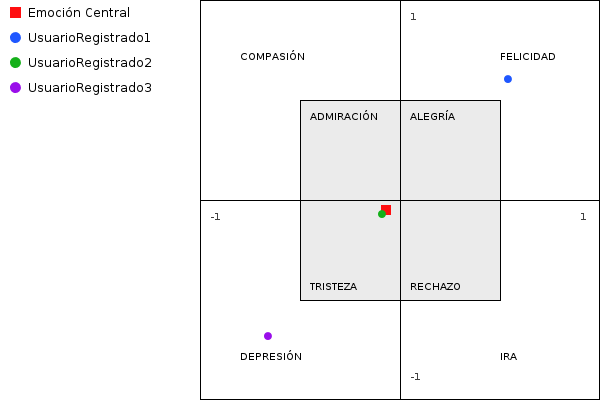
\includegraphics[width=11cm]{ilustraciones/resultados/caso1escenario2-emocioncentral.png}
\end{ilustracion}

\begin{ilustracion}[fuente=\yo, etiqueta=dispersion-emocional-final-caso1escenario2, titulo={Evolución de la Dispersión Emocional ($\sigma(Ag)$), Caso de Estudio 1 Escenario 2}]
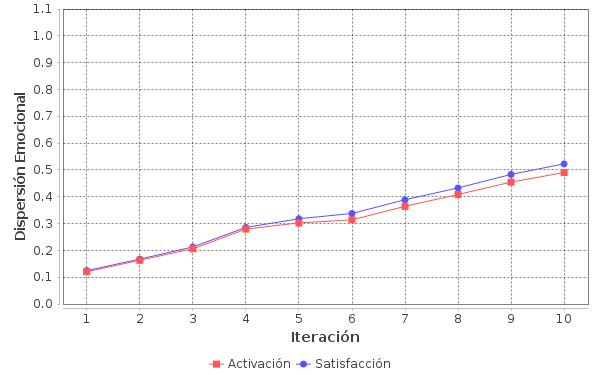
\includegraphics[width=11cm]{ilustraciones/resultados/caso1escenario2-dispersionemocional.png}
\end{ilustracion}

\clearpage
\newpage

\begin{sidewaysfigure}

\begin{cuadro}[etiqueta=resultadoscaso1escenario2, titulo={Evolución de la Emoción Social del Grupo de Agentes ($Ag$), Caso de Estudio 1 Escenario 2}, letra=\tiny]{c|l|l|c|c|l|l|c|c|l|c|c|c|c}
\toprule
\multirow{2}{*}{\textbf{Iteración}} & \multicolumn{6}{c|}{\textbf{Agentes}} &  \multicolumn{3}{c|}{\textbf{$EC(Ag)$}} & \multicolumn{2}{c|}{\textbf{$m(Ag)$}} & \multicolumn{2}{c}{\textbf{$\sigma(Ag)$}} \\ \cline{2-14}
& Nombre & Estímulo & A & S & Emoción & Comportamiento & A & S & Emoción & A & S & A & S \\
\midrule[1pt]
\multirow{3}{*}{0} & UsuarioRegistrado1 & & 0.1 & 0.1 & Alegría & Imitativo & \multirow{3}{*}{0} & \multirow{3}{*}{0} & \multirow{3}{*}{Admiración} & \multirow{3}{*}{0.1} & \multirow{3}{*}{0.1} & \multirow{3}{*}{0.082} & \multirow{3}{*}{0.082}  \\\cline{2-7}
& UsuarioRegistrado2 & & 0 & 0 & Admiración & Imitativo & & & & & & & \\ \cline{2-7}
& UsuarioRegistrado3 & & -0.1 & -0.1 & Tristeza & Cognitivo & & & & & & & \\ \midrule[1pt]
\multirow{3}{*}{1} & UsuarioRegistrado1 & Nueva Edición & 0.13 & 0.14 & Alegría & Imitativo & \multirow{3}{*}{-0.03} & \multirow{3}{*}{-0.027} & \multirow{3}{*}{Tristeza} & \multirow{3}{*}{0.16} & \multirow{3}{*}{0.167} & \multirow{3}{*}{0.12} & \multirow{3}{*}{0.125}  \\\cline{2-7}
& UsuarioRegistrado2 & Artículo Borrado & -0.06 & -0.06 & Tristeza & Cognitivo & & & & & & & \\ \cline{2-7}
& UsuarioRegistrado3 & Artículo Borrado & -0.16 & -0.16 & Tristeza & Cognitivo & & & & & & & \\ \midrule[1pt]
\multirow{3}{*}{2} & UsuarioRegistrado1 & Artículo Nuevo & 0.18 & 0.19 & Alegría & Imitativo & \multirow{3}{*}{-0.017} & \multirow{3}{*}{-0.013} & \multirow{3}{*}{Tristeza} & \multirow{3}{*}{0.203} & \multirow{3}{*}{0.207} & \multirow{3}{*}{0.163} & \multirow{3}{*}{0.167}  \\\cline{2-7}
& UsuarioRegistrado2 & Artículo Nuevo & -0.01 & -0.01 & Tristeza & Cognitivo & & & & & & & \\ \cline{2-7}
& UsuarioRegistrado3 & Artículo Borrado & -0.22 & -0.22 & Tristeza & Cognitivo & & & & & & & \\ \midrule[1pt]
\multirow{3}{*}{3} & UsuarioRegistrado1 & Nueva Edición & 0.21 & 0.23 & Alegría & Imitativo & \multirow{3}{*}{0} & \multirow{3}{*}{0.007} & \multirow{3}{*}{Admiración} & \multirow{3}{*}{0.28} & \multirow{3}{*}{0.287} & \multirow{3}{*}{0.206} & \multirow{3}{*}{0.213}  \\\cline{2-7}
& UsuarioRegistrado2 & Artículo Sobresaliente & 0.07 & 0.07 & Alegría & Imitativo & & & & & & & \\ \cline{2-7}
& UsuarioRegistrado3 & Artículo Borrado & -0.28 & -0.28 & Tristeza & Cognitivo & & & & & & & \\ \midrule[1pt]
\multirow{3}{*}{4} & UsuarioRegistrado1 & Artículo Sobresaliente & 0.29 & 0.31 & Alegría & Imitativo & \multirow{3}{*}{0.027} & \multirow{3}{*}{0.033} & \multirow{3}{*}{Alegría} & \multirow{3}{*}{0.387} & \multirow{3}{*}{0.393} & \multirow{3}{*}{0.279} & \multirow{3}{*}{0.286}  \\\cline{2-7}
& UsuarioRegistrado2 & Artículo Sobresaliente & 0.15 & 0.15 & Alegría & Imitativo & & & & & & & \\ \cline{2-7}
& UsuarioRegistrado3 & Guerra de Ediciones & -0.36 & -0.36 & Tristeza & Cognitivo & & & & & & & \\ \midrule[1pt]
\multirow{3}{*}{5} & UsuarioRegistrado1 & Nueva Edición & 0.32 & 0.35 & Alegría & Imitativo & \multirow{3}{*}{0.04} & \multirow{3}{*}{0.05} & \multirow{3}{*}{Alegría} & \multirow{3}{*}{0.42} & \multirow{3}{*}{0.44} & \multirow{3}{*}{0.302} & \multirow{3}{*}{0.318}  \\\cline{2-7}
& UsuarioRegistrado2 & Nueva Edición & 0.18 & 0.19 & Alegría & Imitativo & & & & & & & \\ \cline{2-7}
& UsuarioRegistrado3 & Artículo Modificado & -0.38 & -0.39 & Tristeza & Cognitivo & & & & & & & \\ \midrule[1pt]
\multirow{3}{*}{6} & UsuarioRegistrado1 & Nueva Edición & 0.35 & 0.39 & Alegría & Imitativo & \multirow{3}{*}{0.023} & \multirow{3}{*}{0.033} & \multirow{3}{*}{Alegría} & \multirow{3}{*}{0.423} & \multirow{3}{*}{0.453} & \multirow{3}{*}{0.314} & \multirow{3}{*}{0.338}  \\\cline{2-7}
& UsuarioRegistrado2 & Artículo Borrado & 0.12 & 0.13 & Alegría & Imitativo & & & & & & & \\ \cline{2-7}
& UsuarioRegistrado3 & Artículo Modificado & -0.4 & -0.42 & Tristeza & Cognitivo & & & & & & & \\ \midrule[1pt]
\multirow{3}{*}{7} & UsuarioRegistrado1 & Artículo Sobresaliente & 0.43 & 0.47 & Alegría & Imitativo & \multirow{3}{*}{0.003} & \multirow{3}{*}{0.013} & \multirow{3}{*}{Alegría} & \multirow{3}{*}{0.463} & \multirow{3}{*}{0.493} & \multirow{3}{*}{0.364} & \multirow{3}{*}{0.389}  \\\cline{2-7}
& UsuarioRegistrado2 & Guerra de Ediciones & 0.04 & 0.05 & Alegría & Imitativo & & & & & & & \\ \cline{2-7}
& UsuarioRegistrado3 & Artículo Borrado & -0.46 & -0.48 & Tristeza & Cognitivo & & & & & & & \\ \midrule[1pt]
\multirow{3}{*}{8} & UsuarioRegistrado1 & Artículo Nuevo & 0.48 & 0.52 & Felicidad & Imitativo & \multirow{3}{*}{-0.027} & \multirow{3}{*}{-0.017} & \multirow{3}{*}{Tristeza} & \multirow{3}{*}{0.507} & \multirow{3}{*}{0.537} & \multirow{3}{*}{0.408} & \multirow{3}{*}{0.433}  \\\cline{2-7}
& UsuarioRegistrado2 & Guerra de Ediciones & -0.04 & -0.03 & Tristeza & Cognitivo & & & & & & & \\ \cline{2-7}
& UsuarioRegistrado3 & Artículo Borrado & -0.52 & -0.54 & Depresión & Reactivo & & & & & & & \\ \midrule[1pt]
\multirow{3}{*}{9} & UsuarioRegistrado1 & Nueva Edición & 0.51 & 0.56 & Felicidad & Imitativo & \multirow{3}{*}{-0.07} & \multirow{3}{*}{-0.057} & \multirow{3}{*}{Tristeza} & \multirow{3}{*}{0.58} & \multirow{3}{*}{0.617} & \multirow{3}{*}{0.455} & \multirow{3}{*}{0.483}  \\\cline{2-7}
& UsuarioRegistrado2 & Guerra de Ediciones & -0.12 & -0.11 & Tristeza & Cognitivo & & & & & & & \\ \cline{2-7}
& UsuarioRegistrado3 & Guerra de Ediciones & -0.6 & -0.62 & Depresión & Reactivo & & & & & & & \\ \midrule[1pt]
\multirow{3}{*}{10} & UsuarioRegistrado1 & Nueva Edición & 0.54 & 0.6 & Felicidad & Imitativo & \multirow{3}{*}{-0.07} & \multirow{3}{*}{-0.05} & \multirow{3}{*}{Tristeza} & \multirow{3}{*}{0.61} & \multirow{3}{*}{0.65} & \multirow{3}{*}{0.49} & \multirow{3}{*}{0.523}  \\\cline{2-7}
& UsuarioRegistrado2 & Nueva Edición & -0.09 & -0.07 & Tristeza & Cognitivo & & & & & & & \\ \cline{2-7}
& UsuarioRegistrado3 & Artículo Borrado & -0.66 & -0.68 & Depresión & Reactivo & & & & & & & \\ \midrule[1pt]
\fuentecuadro{14}{\yo}
\end{cuadro}

\end{sidewaysfigure}

\clearpage
\newpage

\subseccion{Escenario 3: Baja Dispersión Emocional y Alto Número de Agentes}

Como MASOES es una arquitectura que permite modelar
sistemas emergentes y auto-organizados con alta densidad de agentes,
se plantea este escenario con el objetivo de verificar el cálculo de la $ES(Ag)$, con alto
número de agentes y baja dispersión emocional.
Se configura una simulación con 50 agentes emocionales y 20 iteraciones,
e inicializan los estados emocionales de manera aleatoria en todo el modelo afectivo,
y no para una sola emoción. En cada iteracion se envían intencionalmente para todos los agentes, estímulos
que favorecen una emoción positiva (incrementan la reputación de los wikipedistas).

En la \refcuadro{emocion-social-caso1escenario3}, se presentan la $ES(Ag)$ inicial y final.
Con respecto a los valores iniciales, se observa que
la $EC(Ag)$ exhibe Alegría, con $m(Ag)$ y $\sigma(Ag)$ iguales a: (0.98, 1.119) y
(0.59, 0.624), respectivamente. De esto se puede interpretar, que
el grupo de agentes tiene una alta dispersión emocional (emociones muy heterogéneas) al iniciar la simulación,
la \refilustracion{emocion-central-inicial-caso1escenario3} muestra una representación
gráfica del estado inicial.
Los valores finales obtenidos muestran
una disminución en la dispersión emocional,
se obtuvo una $EC(Ag)$ igual a Felicidad: (0.764, 0.829) \refpilustracion{emocion-central-final-caso1escenario3},
con $m(Ag)$ igual a: (0.697, 0.755) y una $\sigma(Ag)$
de (0.305, 0.293).
Es importante resaltar, que para realizar una interpretación adecuada de la $ES(Ag)$,
es necesario analizar sus componentes ($EC(Ag)$,  $m(Ag)$ y $\sigma(Ag)$), sobre todo la $\sigma(Ag)$.
Para este caso, aunque la $EC(Ag)$ inicial fue Alegría, pocos agentes mostraban dicha emoción,
pero al finalizar la simulación, la mayoría de los agentes si exhibían Felicidad
tal como la $EC(Ag)$, y se debe a una disminución en la $\sigma(Ag)$, en otras palabras,
los estados emocionales de los agentes se aproximaron,
esto puede ser apreciado en \refilustracion{dispersion-emocional-final-caso1escenario3}.
Los valores resultantes develan la importancia que representa la $\sigma(Ag)$ para
la propuesta de $ES(Ag)$ presentada en este trabajo.

Otro aspecto interesante en la simulación, es que en los estados emocionales finales
algunos de los agentes tuvieron una activación o satisfacción igual a 1, esto se debe a que solo
recibieron estímulos que propician emociones positivas y sus estados emocionales llegaron al límite
del modelo afectivo.

\begin{cuadro}[etiqueta=emocion-social-caso1escenario3, titulo={Valor Inicial y Final de la Emoción Social del Grupo de Agentes ($Ag$), Caso 1 Escenario 3}]{llll}
\toprule
 &  $EC(Ag)$ & $m(Ag)$ & $\sigma(Ag)$ \\
\midrule
Inicial & (0.001, 0.125) Alegría & (0.98, 1.119) & (0.59, 0.624) \\
Final & (0.764, 0.829) Felicidad & (0.697, 0.755) & (0.305, 0.293) \\
\bottomrule
\fuentecuadro{4}{\yo}
\end{cuadro}

\begin{ilustracion}[fuente=\yo, etiqueta=emocion-central-inicial-caso1escenario3, titulo={Emoción Central Inicial, Caso de Estudio 1 Escenario 3}]
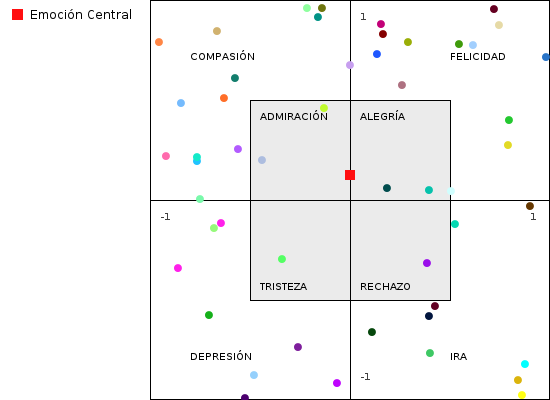
\includegraphics[width=10cm]{ilustraciones/resultados/caso1escenario3-emocioncentral-inicial.png}
\end{ilustracion}

\begin{ilustracion}[fuente=\yo, etiqueta=emocion-central-final-caso1escenario3, titulo={Emoción Central Final, Caso de Estudio 1 Escenario 3}]
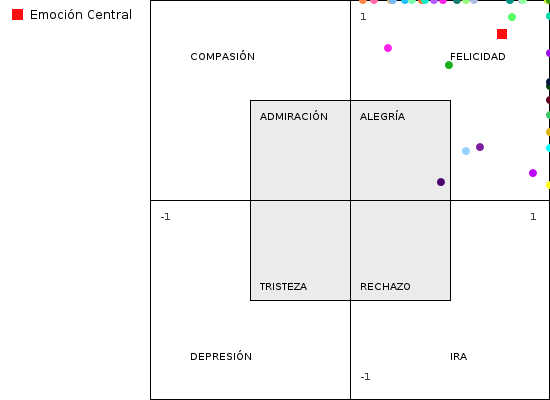
\includegraphics[width=10cm]{ilustraciones/resultados/caso1escenario3-emocioncentral-final.png}
\end{ilustracion}

\begin{ilustracion}[fuente=\yo, etiqueta=dispersion-emocional-final-caso1escenario3, titulo={Evolución de la Dispersión Emocional ($\sigma(Ag)$), Caso de Estudio 1 Escenario 3}]
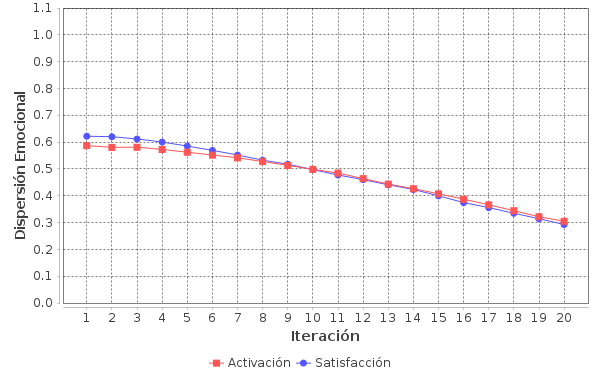
\includegraphics[width=11cm]{ilustraciones/resultados/caso1escenario3-dispersionemocional.png}
\end{ilustracion}

\clearpage
\newpage

\subseccion{Escenario 4: Alta Dispersión Emocional y Alto Número de Agentes}

Siguiendo la misma idea que el escenario anterior,
para este se configura una simulación con 50 agentes emocionales y 20 iteraciones,
e inicializan los estados emocionales de manera aleatoria en todo el modelo afectivo,
no obstante, se envían estímulos que incrementan la reputación al 50\%
de los wikipedistas (25 agentes) y estímulos que decrementan la reputación al otro 50\%,
con el objetivo de verificar la generación de la $ES(Ag)$ en un grupo con alto
número de agentes y alta $\sigma(Ag)$.

Los resultados obtenidos \refpcuadro{emocion-social-caso1escenario4},
muestran que la $EC(Ag)$ se modificó ligeramente pasando de (-0.138, -0.142)
a (-0.076, -0.067), manteniéndose en Tristeza,
lo interesante en este escenario es el resultado
obtenido en la $\sigma(Ag)$, como se muestra en la \refilustracion{dispersion-emocional-final-caso1escenario4},
se incrementó tanto para la activación como para la satisfacción, debido
a que los estados emocionales se fueron distanciando (muy heterogéneos), aun así
la $EC(Ag)$ se mantuvo en Tristeza. Una de las conclusiones para esto,
es que el número de agentes no influye en el resultado de la $EC(Ag)$,
más la $\sigma(Ag)$ si es un factor importante a tomar en cuenta a la hora
de hacer una interpretación. Además, se puede observar en la
\refilustracion{emocion-central-inicial-caso1escenario4} como los estados emocionales de los
agentes se distribuyen por todo el modelo afectivo al iniciar la simulación,
y al finalizarla los agentes se
concentraron en los cuadrantes 1 (Alegría y Felicidad)
y 4 (Tristeza y Depresión) como se muestra en la \refilustracion{emocion-central-final-caso1escenario4},
es decir, dos grupos. Esto abre una oportunidad de investigación futura, en la que se puedan generar más de una
$ES(Ag)$ dependiendo del número de agrupaciones de estados emocionales exhibidos.

De igual manera que el escenario anterior,
para algunos de los agentes se obtuvo una activación o satisfacción igual a 1 o -1 en el resultado final,
esto se debe a que solo recibieron un tipo de estímulos, que incrementa o decrementa la reputación,
y los estados emocionales llegaron al valor mínimo o máximo permitido según el modelo afectivo de MASOES.

\begin{cuadro}[etiqueta=emocion-social-caso1escenario4, titulo={Valor Inicial y Final de la Emoción Social del Grupo de Agentes ($Ag$), Caso 1 Escenario 4}]{llll}
\toprule
 &  $EC(Ag)$ & $m(Ag)$ & $\sigma(Ag)$ \\
\midrule
Inicial & (-0.138, -0.142) Tristeza & (1.051, 1.115) & (0.598, 0.652) \\
Final & (-0.076, -0.067) Tristeza & (1.076, 1.067) & (0.831, 0.743) \\
\bottomrule
\fuentecuadro{4}{\yo}
\end{cuadro}

\begin{ilustracion}[fuente=\yo, etiqueta=emocion-central-inicial-caso1escenario4, titulo={Emoción Central Inicial, Caso de Estudio 1 Escenario 4}]
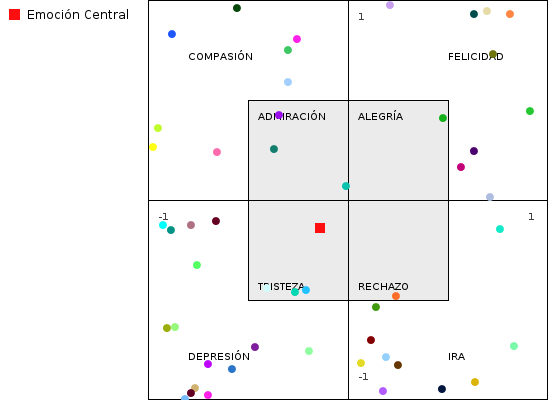
\includegraphics[width=10cm]{ilustraciones/resultados/caso1escenario4-emocioncentral-inicial.png}
\end{ilustracion}

\begin{ilustracion}[fuente=\yo, etiqueta=emocion-central-final-caso1escenario4, titulo={Emoción Central Final, Caso de Estudio 1 Escenario 4}]
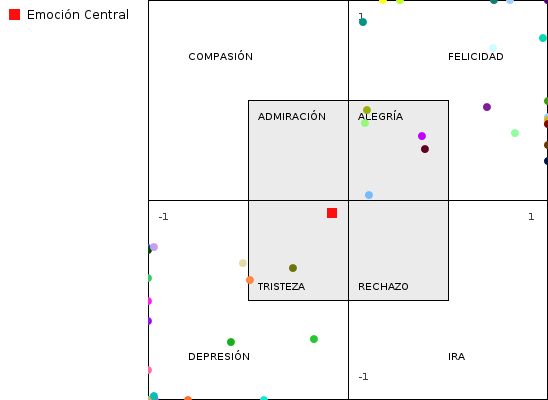
\includegraphics[width=10cm]{ilustraciones/resultados/caso1escenario4-emocioncentral-final.png}
\end{ilustracion}

\begin{ilustracion}[fuente=\yo, etiqueta=dispersion-emocional-final-caso1escenario4, titulo={Evolución de la Dispersión Emocional ($\sigma(Ag)$), Caso de Estudio 1 Escenario 4}]
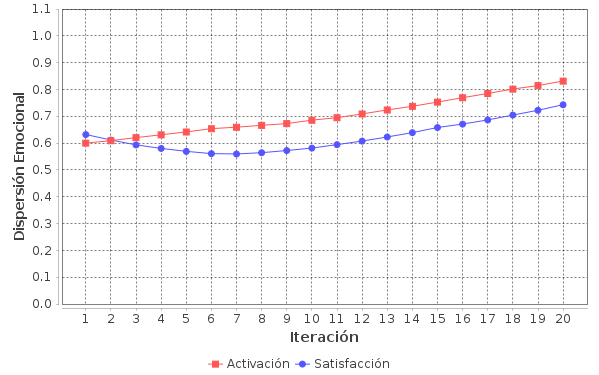
\includegraphics[width=11cm]{ilustraciones/resultados/caso1escenario4-dispersionemocional.png}
\end{ilustracion}

\clearpage
\newpage

\seccion{Caso de Estudio 2: Emociones a Nivel Individual}

El objetivo de este caso de estudio es verificar que el modelo afectivo propuesto en
MASOES a nivel de implementación, genere correctamente emociones positivas y negativas
individualmente en los agentes emocionales. A través de dos escenarios atómicos,
se generarán emociones y se comparará los resultados con los obtenidos
a nivel de diseño en \cite{perozo2012}.
Para esto se realiza una simulación en ambos escenarios con un agente de tipo Usuario Registrado
y 20 iteraciones.

\subseccion{Escenario 1: Grado de Satisfacción Alto y Activación Alto, Medio y Bajo}

Para este escenario, un colaborador propone y desarrolla un contenido, recibiendo
un incremento de reputación por la calidad del aporte realizado. Este usuario
podría experimentar un alto grado de satisfacción y activación, que se
traduciría en emociones positivas individuales, lo que conllevaría a un
comportamiento imitativo para tratar de repetir esta experiencia,
de acuerdo al modelo afectivo de MASOES. Esto se debe a que según el espacio afectivo definido
\refpilustracion{modelo-afectivo}, al permanecer alto el grado de satisfacción
del agente y variar el grado de activación, se siguen promoviendo las emociones
positivas, bien sean individuales o sociales (cuadrantes 1 y 2 del espacio
afectivo bidimensional). Por lo dicho anteriormente, se seleccionan
solo estímulos que incrementan la reputación del agente \refpcuadro{estimulos-propuestos}.
Se inicializa el agente con un satisfacción igual a 1, ya que, se tiene como objetivo observar la evolución del estado emocional
siendo afectado únicamente por la activación, y se asigna una activación baja de -0.6,
estos valores corresponden a la emoción Compasión.

Sobre los resultados, en la \refilustracion{emociones-individuales-escenerio1-estado-emocional-colaborador1} se observa que
aunque la satisfacción se mantiene constante, la activación se incrementó.
A su vez,
en la \refilustracion{emociones-individuales-escenario1-modificacion-de-emociones}, se refleja que
la emoción asociada al estado actual del agente fue modificándose a medida que la activación iba
en incremento, pasando de compasión a felicidad y la \refilustracion{emociones-individuales-escenario1-modificacion-de-comportamiento},
muestra que el agente se mantuvo con un comportamiento imitativo.

Los resultados obtenidos permiten verificar que
la implementación cumple con lo elaborado a nivel de diseño \citep{perozo2012}, al permanecer alto el grado de satisfacción del
agente y variar el grado de activación, se siguen promoviendo las emociones positivas,
bien sean individuales o sociales. En
otras palabras, a pesar de variar el grado de activación y producir emociones menos o
más intensas, el agente mantuvo su comportamiento imitativo.

\begin{ilustracion}[fuente=\yo, etiqueta=emociones-individuales-escenerio1-estado-emocional-colaborador1, titulo={Variación del Estado Emocional del Agente, Caso de Estudio 2 Escenario 1}]
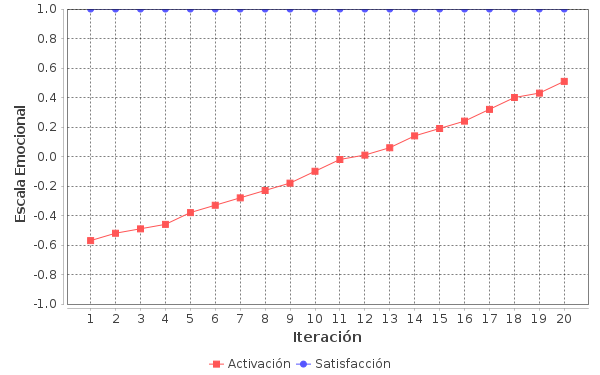
\includegraphics[width=11cm]{ilustraciones/resultados/caso2escenerio1-estado-emocional-colaborador1.png}
\end{ilustracion}

\begin{ilustracion}[fuente=\yo, etiqueta=emociones-individuales-escenario1-modificacion-de-emociones, titulo={Variación de la Emoción Exhibida por el Agente, Caso de Estudio 2 Escenario 1}]
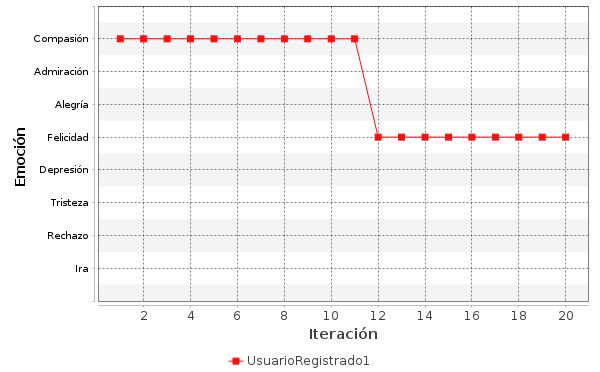
\includegraphics[width=11cm]{ilustraciones/resultados/caso2escenerio1-modificacion-de-emociones.png}
\end{ilustracion}

\begin{ilustracion}[fuente=\yo, etiqueta=emociones-individuales-escenario1-modificacion-de-comportamiento, titulo={Variación del Comportamiento Exhibido por el Agente, Caso de Estudio 2 Escenario 1}]
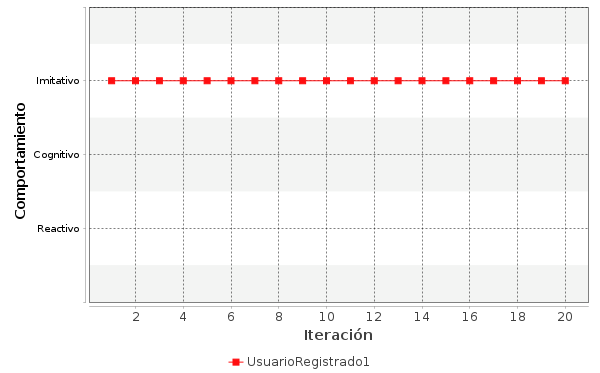
\includegraphics[width=11cm]{ilustraciones/resultados/caso2escenerio1-modificacion-de-comportamiento.png}
\end{ilustracion}

\clearpage
\newpage

\subseccion{Escenario 2: Grado de Satisfacción y Activación Medio y Bajo}

A diferencia de lo anterior, en este escenario un usuario registrado propone y desarrolla un contenido,
el cual amerita modificaciones por la comunidad, recibiendo
un decremento de reputación por el aporte realizado. Este usuario
podría experimentar disminución del grado de satisfacción y activación,
provocándole emociones negativas y activando un comportamiento
cognitivo o reactivo.
Se seleccionan
solo estímulos que decrementan la reputación del agente \refpcuadro{estimulos-propuestos}.
El agente es inicializado en la emoción Alegría con una activación de 0.5
y satisfacción 0.3.

Con respecto a los resultados, en la \refilustracion{emociones-individuales-escenerio2-estado-emocional-colaborador1}, se puede observar
la disminución en la activación y satisfacción del estado emocional del agente.
Los resultados reflejan que el agente varió su emoción pasando de alegría a rechazo, tristeza y depresión \refpilustracion{emociones-individuales-escenario2-modificacion-de-emociones}.
Así mismo, la \refilustracion{emociones-individuales-escenario2-modificacion-de-comportamiento}
muestra la variación de comportamientos del agente, el cual inició con comportamiento imitativo
pero fue actualizado a un comportamiento de tipo cognitivo y posteriormente uno reactivo.
Estos valores concuerdan con los escenarios 2 y 3 expuestos
en \cite{perozo2012}, la disminución de reputación en el agente afectará tanto la activación
como la satisfacción de su estado emocional,
provocándole emociones negativas y activando un comportamiento
reactivo o cognitivo.

\begin{ilustracion}[fuente=\yo, etiqueta=emociones-individuales-escenerio2-estado-emocional-colaborador1, titulo={Variación del Estado Emocional del Agente, Caso de Estudio 2 Escenario 2}]
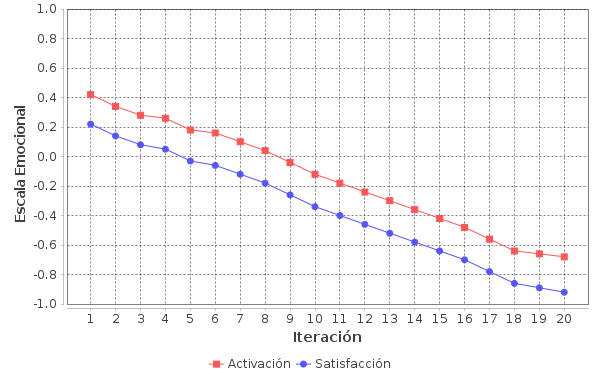
\includegraphics[width=11cm]{ilustraciones/resultados/caso2escenerio2-estado-emocional-colaborador1.png}
\end{ilustracion}

\begin{ilustracion}[fuente=\yo, etiqueta=emociones-individuales-escenario2-modificacion-de-emociones, titulo={Variación de la Emoción Exhibida por el Agente, Caso de Estudio 2 Escenario 2}]
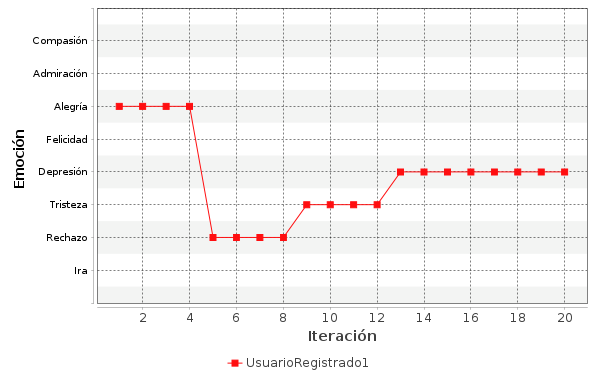
\includegraphics[width=11cm]{ilustraciones/resultados/caso2escenerio2-modificacion-de-emociones.png}
\end{ilustracion}

\begin{ilustracion}[fuente=\yo, etiqueta=emociones-individuales-escenario2-modificacion-de-comportamiento, titulo={Variación del Comportamiento Exhibido por el Agente, Caso de Estudio 2 Escenario 2}]
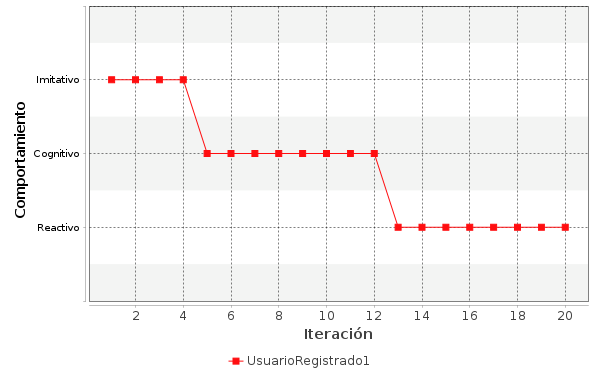
\includegraphics[width=11cm]{ilustraciones/resultados/caso2escenerio2-modificacion-de-comportamiento.png}
\end{ilustracion}

  	%%
% Copyright (c) 2017 Saúl Piña <sauljabin@gmail.com>.
%
% This program is free software: you can redistribute it and/or modify
% it under the terms of the GNU General Public License as published by
% the Free Software Foundation, either version 3 of the License, or
% (at your option) any later version.
%
% This program is distributed in the hope that it will be useful,
% but WITHOUT ANY WARRANTY; without even the implied warranty of
% MERCHANTABILITY or FITNESS FOR A PARTICULAR PURPOSE.  See the
% GNU General Public License for more details.
%
% You should have received a copy of the GNU General Public License
% along with this program.  If not, see <http://www.gnu.org/licenses/>.
%%

\capitulo{Conclusiones y Recomendaciones}

La arquitectura multiagente MASOES permite modelar un sistema emergente
y auto-organizado. Esta arquitectura
describe los elementos y relaciones a nivel individual y colectivo, que
determinan los fenómenos de emergencia y auto-organización en un sistema.
En este trabajo se abordó la implementación del modelo afectivo
propuesto en MASOES, y por ende su componente conductual,
el cual permite generar cambios dinámicos de comportamientos en los
agentes emocionales, guiados por su estado emocional.
Adicionalmente, se propone el cálculo de
la Emoción Social de un grupo de agentes,
que se compone por un conjunto de tres valores: la Emoción Central,
que determina la emoción que tienden a exhibir los agentes;
la Distancia Máxima, determina los estados emocionales más alejados del grupo;
y la Dispersión Emocional, que define la variación de estados emocionales del grupo,
es decir, dicta si los estados emocionales son homegéneos o heterogéneos.

A fin de verificar que la implementación del modelo afectivo genere correctamente emociones a nivel individual y colectivo
y que la priorización de los tipos de comportamiento sea acorde a las reglas de MASOES,
se desarrollaron casos de estudio
basados en lo modelado por \cite{perozo2012} sobre el sistema colaborativo Wikipedia.
Los resultados obtenidos demuestran que la implementación cumple
con lo especificado en MASOES, tanto a nivel individual como colectivo.
Uno de los hallazgos interesantes es la importancia que tiene la dispersión emocional
sobre la interpretación de la emoción central, esto se debe, a que
expresa cuan representativa es la emoción central frente a un grupo de agentes.
Se pudo comprobar que la emoción central es más válida a medida que la dispersión
emocional es más cercana a cero, ya que se trata de un conjunto de agentes que tienen emociones muy parecidas (homogéneas).
También, se observó que el número de agentes no influye directamente en el resultado
e interpretación de la emoción central, en otras palabras, si un grupo de agentes
es pequeño los resultados de la emoción central se comportarán de la misma forma que en
un grupo de agentes grande.
A nivel individual,
se pudo observar que los agentes generan emociones y priorizan los comportamientos
correctamente, esto se hizo a través de la comparación de los resultados
con los obtenidos a nivel de diseño \citep{perozo2012}, los cuales concuerdan inequívocamente.

Con respecto a los aportes, este trabajo de investigación no solo
provee una implementación del modelo afectivo de MASOES, sino que también,
proporciona un marco de trabajo el cual se puede seguir extendiendo,
para simular cualquier tipo de sistema emergente y auto-organizado modelado con MASOES.
Por otro lado, se construyeron diferentes utilitarios de código que permiten,
entre otras cosas, controlar la plataforma JADE, comunicar agentes, realizar pruebas funcionales y
trabajar con el lenguaje \textit{Prolog}, también, se incluyeron interfaces gráficas
que sirven para el monitoreo de agentes o para la configuración de simulaciones.
Es importante destacar que dichas interfaces pueden ser modificadas, para
adaptarse a diferentes dominios y sistemas.
La interfaz de configuración de simulación permite observar gráficos en tiempo real
acerca de la emoción social y los estados emocionales individuales de cada agente,
además, incluye la generación de resultados a través de archivos de texto.
Se desarrolló un agente que calcula la emoción social.
Este cálculo se basa en el promedio de los estados emocionales de un grupo de agentes y
la desviación estándar de dicho promedio. La emoción social es de gran importancia,
ya que describe la tendencia de los estados emocionales de un grupo de agentes,
y los agentes emocionales podrían utilizarla como herramienta para cumplir
sus objetivos colectivos.

Otro de los aportes más relevantes de este trabajo, es el diseño de una ontología de
comunicación para MASOES, específicamente para agentes estandarizados FIPA, con ella
es posible comunicar los agentes emocionales entre sí o con otros tipos de agentes,
además, es posible una comunicación entre diferentes plataformas,
es decir, los agentes escritos en lenguaje \textit{Java} pueden comunicarse
con agentes programados en lenguajes diferentes.

Otro aporte interesante, es la implementación y diseño de la Base de Conocimiento
Conductual, esta fue desarrollada con el lenguaje de programación \textit{Prolog},
ampliamente utilizado por su versatilidad y facilidad de uso, para esto
se propuso una manera estándar de definir el conocimiento asociado
al agente, a los tipos de emociones, a la priorización de comportamiento y a los estímulos,
este último de gran importancia para los agentes emocionales, ya que estos
pueden y deben registrar como afectan los estímulos a su estado emocional.
En cada estímulo se deben establecer los parámetros
que definen el incremento de la activación y satisfacción del estado emocional del agente.
A su vez, se propone un algoritmo para la
actualización del estado emocional del agente de manera incremental.

Es importante destacar, que la implementación se llevó a cabo tomando en cuenta los estándares FIPA,
lo que permite la interoperabilidad de los agentes emocionales con cualquier otro agente FIPA,
esto hace que sea estándar y fácil de extender por otros.

Como trabajo futuro, se podría implementar otros componentes individuales de la arquitectura de MASOES,
como son, los componentes Cognitivo, Reactivo y Social, y componentes colectivos como
la Base de Conocimiento Colectivo, todo esto con la finalidad de completar la implementación
de esta arquitectura y ser usada para modelar e instanciar un sistema colectivo
emergente y auto-organizado de software. Asimismo, se puede destacar que el componente conductual
presentado en este trabjao, es susceptible a modificaciones y mejoras, como por ejemplo:
se podría mejorar el diseño de clases o utilizar un lenguaje lógico diferente de \textit{Prolog}
para construir la Base de Conocimiento Conductual, o también, incluir más conocimiento
en dicha base.
Otra oportunidad de investigación, es proponer un cálculo de emoción social,
que pueda dar como resultado más de una emoción central, esto, basado en las agrupaciones de estados emocionales
que puedan emerger en el grupo de agentes, ya que como se vio, la interpretación de la emoción central propuesta
en este trabajo está sujeta al resultado de la dispersión emocional y en menor manera a la distancia máxima.

Por otra parte, sería interesante probar la implementación propuesta en este trabajo
en diferentes host, en otras palabras, que los agentes no se instancien localmente, sino
que se instancien y comuniquen en una red, lo cual sería útil en áreas como la robótica,
donde cada agente emocional sea un robot y este modifique su comportamiento
según su estado emocional, para esta propuesta se recomienda implementar previamente
al menos los componentes Cognitivo y Reactivo de MASOES.

  \end{contenido}

  \hacerbibliografia

%  \begin{anexos}
%  	%%
% Copyright (c) 2017 Saúl Piña <sauljabin@gmail.com>.
%
% This program is free software: you can redistribute it and/or modify
% it under the terms of the GNU General Public License as published by
% the Free Software Foundation, either version 3 of the License, or
% (at your option) any later version.
%
% This program is distributed in the hope that it will be useful,
% but WITHOUT ANY WARRANTY; without even the implied warranty of
% MERCHANTABILITY or FITNESS FOR A PARTICULAR PURPOSE.  See the
% GNU General Public License for more details.
%
% You should have received a copy of the GNU General Public License
% along with this program.  If not, see <http://www.gnu.org/licenses/>.
%%

\anexo{Curriculum Vitae}

\anexo{Instrumento de Recolección de Datos}

%  \end{anexos}

\end{document}
